 	
\documentclass[tugasakhir,satusetengahspasi]{skripsidtntf}

\usepackage{amsmath}
\usepackage{amssymb}
\usepackage{amscd}
\usepackage{amstext}
\usepackage{lipsum}
\usepackage{placeins}
\usepackage{pdflscape}

\judul{Perancangan Kontroler Lingkungan Termal \textit{Climate Chamber} Berbasis Jaringan Saraf Tiruan}

\juduleng{Design of ANN Based Controller for Thermal Environment Climate Chamber}

\permasalahan{ Untuk memenuhi kebutuhan penelitian kenyamanan termal, kondisi lingkungan termal pada \textit{climate chamber} (sebagai ruang uji termal) haruslah dapat dikondisikan secara otomatis sesuai dengan skema pengujian penelitian.
}

\jenisTA{SKRIPSI}
\gelar{Sarjana S-1}
\prodi{Teknik Fisika}  % Teknik Nuklir atau Teknik Fisika
\prodieng{Engineering Physics}  %   Nuclear Engineering atau Engineering Physics 
\jurusan{Teknik Nuklir dan Teknik Fisika}
\nama{Ridhan Fadhilah}
\nim{15/384859/TK/43521}
\angkatan{2015}
\thselesai{2020}
\tglujian{26 Agustus 2020}
\tglujianeng{August 26th, 2020}
\tglpenulisan{\textcolor{red}{....}}

\pembimbingutama{Faridah, S.T., M.Sc.}
\nippembimbingutama{19760214 200212 2 001}
\pembimbingpendamping{Ir. Agus Arif, M.T.}
\nippembimbingpendamping{196608122 199303 1 004}

\ketuasidang{Faridah, S.T., M.Sc.}
\nipketuasidang{19760214 200212 2 001}
\pengujiutama{Dwi Joko Suroso, S.T., M.Eng.}
\nippengujiutama{11119880 820170 6 101}
\anggotapenguji{Sentagi Sesotya Utami, S.T., M.Sc., Ph.D.}
\nipanggotapenguji{19750226 200212 2 002}

\kadep{Nopriadi, S.T., M.Sc. Ph.D}
\nipkadep{19731119 200212 1 002}




\begin{document}

%\halamansampul
\halamanjudul
\halamanpernyataan
\halamanpengesahan
\halamantugas

\persembahan
\begin{center}
\emph{ Karya ini ku persembahkan untuk kedua orang tua, adik, keluarga, dan kerabat dekat. Terima kasih atas segala dukungan dan doa yang kalian berikan.}
\end{center}


\motto
%\begin{center}
%    $\ldots$ Hiduplah seperti kayu jati. Semakin tua semakin punya jati diri. $\ldots$
%\end{center}

\noindent \emph{\\"The amateur waits for inspiration. \\
	The professional knows that it will come after he starts."}
\begin{flushright}
	- Steven Pressfield
\end{flushright}


%\noindent \emph{\\ \\"Knowledge is not power…it’s potential power. \\ Execution will trump knowledge any day."}

%\begin{flushright}
%	- Tony Robbins
%\end{flushright}

%\noindent \emph{\\ \\"I have been impressed with the urgency of doing. \\ Knowing is not enough; we must apply.\\ Being willing is not enough; we must do."}

%\begin{flushright}
%	- Leonardo Da Vinci
%\end{flushright}


\pengantar
Puji dan syukur penulis panjatkan kehadirat Allah SWT yang telah memberi-kan rahmat dan karunia-Nya, sehingga penulis dapat menyelesaikan tugas akhir beserta penulisan skripsi ini untuk memenuhi sebagian persyaratan untuk memperoleh gelar sarjana teknik fisika.

Dalam pembuatan skripsi ini banyak kesulitan yang penulis alami terutama disebabkan oleh kurangnya pengetahuan dan sumber-sumber informasi yang terbatas. Namun berkat bimbingan dan bantuan dari semua pihak akhirnya skripsi ini dapat terselesaikan tepat pada waktunya. Oleh karena itu, penulis mengucapkan terima kasih kepada semua pihak yang telah mengarahkan dan membantu penulis dalam penyusunan skripsi ini, khususnya kepada:

\begin{enumerate}
	\item Allah SWT, atas berkat dan rahmat-Nya akhirnya penulis senantiasa diberikan kekuatan, ketabahan, dan ketenangan dalam menjalani lika-liku kehidupan.
	\item Ayah dan Ibu yang telah membesarkan, mendidik, memberikan semangat, serta doa yang tak pernah henti sehingga penulis terus bersemangat dalam menjalani kehidupan, khususnya dalam pengerjaan tugas akhir ini.
	\item Ibu Faridah selaku pembimbing utama penulis yang senantiasa memberikan masukan, arahan, dan semangat dalam mengerjakan serta menyelesaikan tugas akhir ini.
	\item Bapak Agus Arif selaku pembimbing kedua penulis yang telah memberikan masukan, arahan, dan semangat dalam mengerjakan serta menyelesaikan tugas akhir ini.
	\item Bapak Nopriadi selaku dosen pembimbing akademik penulis yang senansitasa memberikan masukan, arahan dan semangat dalam menjalani perkuliahan.
	\item Seluruh Dosen dan Staf Departemen Teknik Nuklir dan Teknik Fisika Fakultas Teknik Universitas Gadjah Mada (DTNTF FT-UGM).
	\item Kerabat-kerabat dekat penulis, yakni M. Faisal Al Bantani, Salsabila K. Khansa, M. N. Fathurrahman, M. Aldan H. A., dan Irfanda Husni Sahid.	
	\item Tim TA kerabat Lab SSTK yakni Armand, Fathan, Ivan, Yerico, Shaki, Yogi, Didik, Radit, Muna, Tanto, dan Faisal.
	\item Teman-teman TF C 2015 yang senantiasa menjadi teman seperjuangan dalam menjalani kuliah selama lebih kurang 4 tahun di DTNTF FT-UGM.
	\item Serta masih banyak lagi berbagai pihak yang tidak dapat penulis sebutkan satu persatu.
\end{enumerate}

Pepatah bilang "tak ada gading yang tak retak", begitu pula dengan penulisan ini. Penulisan yang masih jauh dari kata sempurna. Oleh karena itu, penulis me-mohon maaf apabila terdapat kekurangan ataupun kesalahan yang tertera pada skripsi ini. Kritik dan saran sangat diharapkan agar penulis dapat menulis lebih baik serta berdaya guna dimasa yang akan datang.
\newline

\begin{flushright}
Yogyakarta, Agustus 2020
\end{flushright}
% %
\vspace{0.5cm}
\begin{flushright}
Ridhan Fadhilah
\end{flushright}

\tableofcontents

\listoftables

\listoffigures

%\input{simbol}
\lambang
% PErhatikan urutan abjad kode nomenclature, misal abg, abh, cbe, cbi, menyatakan urutan penulisan di hasil akhir file .pdf. 
%Lihat contoh untuk Singkatan, meskipun urutan penulisan tidak urut abjad, misal ebh mendahului ebe, tetapi hasil akhirnya tetap urut abjad.

% LAMBANG ROMAWI
\nomenclature[aaa]{T${_{db}}$}{Suhu Ruang (\textit{Dry-Bulb Temperature})  \nomunit{$^\circ$C}}
\nomenclature[aab]{RH}{Kelembapan Relatif  \nomunit{\%}}
\nomenclature[aac]{T$_o$}{Suhu Lingkungan (\textit{Dry-Bulb Temeperature}) \nomunit{$^\circ$C}}
\nomenclature[aad]{RD}{Intensitas Radiasi Matahari  \nomunit{W/m$^2$}}
\nomenclature[aae]{AC}{\textit{Setting} AC \nomunit{$^\circ$C}}
\nomenclature[aaf]{HT}{Banyak \textit{heater} menyala \nomunit{ON}}
\nomenclature[aag]{$t$}{Waktu \nomunit{detik}}
\nomenclature[aah]{$f$}{Frekuensi \nomunit{Hertz}}
\nomenclature[aai]{R}{Koefisien Korelasi \nomunit{\%}}
\nomenclature[aaj]{$\mathbb{R}$}{Domain Bilangan Riil}
\nomenclature[aak]{$R(s)$}{Masukan Sistem Kontrol}
\nomenclature[aal]{$C(s)$}{Keluaran Sistem Kontrol}
\nomenclature[aam]{$E(s)$}{Galat Sistem Kontrol}
\nomenclature[aan]{$K$}{Konstanta Pengali}
\nomenclature[aao]{$T(s)$}{Fungsi Pengali Kalang Tertutup}
\nomenclature[aap]{$G(s)$}{Fungsi Pengali Kalang Tertutup Umpan Balik Satuan}
\nomenclature[aar]{$x$}{Lapisan Masukan Jaringan Saraf Tiruan}
\nomenclature[aas]{$y$}{Lapisan Keluaran Jaringan Saraf Tiruan}
\nomenclature[aat]{$z$}{Lapisan Tersembunyi Jaringan Saraf Tiruan}
\nomenclature[abz]{}{}
\nomenclature[aaz]{}{}

% LAMBANG YUNANI
\nomenclature[bba]{$\nu$}{Bobot Jaringan Saraf Tiruan}
\nomenclature[bbt]{$\sigma$}{Fungsi Aktivasi Neuron}

% SUBSKRIP
%\nomenclature[cba]{i}{Iterasi Lapisan Tersembunyi}
%\nomenclature[cbb]{j}{Iterasi Input}
%\nomenclature[cbc]{l}{Iterasi Neuron}
\nomenclature[cbd]{\textit{steady-state}}{Kondisi-Ajeg}

% SUPERSKRIP
\nomenclature[dbj]{n}{Dimensi n}
\nomenclature[dbk]{T}{Fungsi Tranpos Vektor/Matriks}

% SINGKATAN
\nomenclature[eaa]{ANN}{\textit{Artificial Neural Network}}
\nomenclature[eab]{DBT}{\textit{Dry-Bulb Temperature}}
\nomenclature[eae]{IES-VE}{\textit{Integrated Environmental Solutions - Virtual Environment}}
\nomenclature[eaf]{DTNTF}{Departemen Teknik Nuklir dan Teknik Fisika}
\nomenclature[eag]{JST}{Jaringan Saraf Tiruan}
\nomenclature[eah]{MRT}{\textit{Mean Radiant Temperature}}
\nomenclature[eai]{MAE}{\textit{Mean Absoulte Error}}
\nomenclature[eaj]{MSE}{\textit{Mean Squared Error}}
\nomenclature[eak]{NN}{\textit{Neural Network}}



\begin{intisari}
% Ganti perintah \lipsum dengan isi intisari.
\lipsum[100-101]

\vspace{0.5cm}
\hspace{-1.2cm}
\textbf{Kata kunci}: Lingkungan Termal, Sistem Kontrol, Jaringan Saraf Tiruan, Ruang Iklim.



\end{intisari}

\begin{abstracteng}
% ganti perintah \lipsum dengan isi abstract
Thermal comfort studies require the thermal environment conditions in the climate chamber (as a thermal test room) to be automatically conditioned according to the research test scheme. Climate chamber can be realized if the climatic conditions in it can be controlled according to the needs of the research scenario. Therefore, we need a control system capable of controlling the thermal environment in the climate chamber. 

This study uses a sample of 24,000 data obtained from the IES-VE simulation. By using this data, a controller based on an artificial neural network (ANN) was built to control air temperature (T$_{db}$) and relative humidity (RH) in the climate chamber. The Controller is designed from ANN model using the principle of plant inverse model based on IES-VE simulation data. Controller was designed by varying the distribution of training data, activation functions, and many neurons in the hidden layer. The model is selected based on the smallest mean squared error from the variation in the model. The control simulation is carried out with a heating scenario with a rate of 0.625$^\circ$C. %The performance of the simulation results is reviewed through the steady-state error value.

The Controller was built using MATLAB and simulated using Simulink. The ANN Controller was created by spliting the data into 80\% training data, 10\% validation data, and 10\% testing data. The ANN controller uses the hyperbolic tangent activation function. The ANN Controller has a network architecture with one hidden layer containing 35 neurons. The results of the design able to control the thermal environment of the climate chamber with a steady-state error value 0.18$^\circ$C for room temperature. However, the controller is not able to control the room temperature of climate chamber above the set point value of 26$^\circ$C because of the thermal environment data from the IES-VE Model does not represent the system conditions at high temperatures.
%\lipsum[148-149]

\vspace{0.4cm}
\hspace{-1.2cm}
\textbf{Keywords}: Thermal Environment, Controller, Neural Network, Climate Chamber.



\end{abstracteng}


\chapter{PENDAHULUAN}\label{pendahuluan}
\section{Latar Belakang}\label{latar belakang}

Indonesia merupakan pengguna energi terbesar di Asia Tenggara, yaitu lebih dari 36\% penggunaan energi primer Asia Tenggara. Antara tahun 2000 dan 2015, produk domestik bruto (PDB) Indonesia bertambah dua kali lipat dan kebutuhan listrik meningkat 150\%. Pertumbuhan ekonomi mendorong kebutuhan energi Indonesia. Pengguna energi terbesar Indonesia tahun
2015 adalah sektor rumah tangga (38\%) dan industri dan jasa (29\%), diikuti oleh transportasi (27\%) (Gambar\ref{fig:1:energy}).
\begin{figure}[!h]
	\centering
	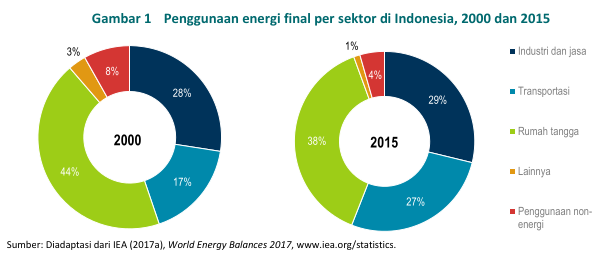
\includegraphics[width=1\textwidth]{figures/EnergyUsage}
	\caption{Penggunaan energi final per sektor di Indonesia, 2000 dan 2015}
	\label{fig:1:energy}
\end{figure}
Efisiensi sangat penting dilakukan untuk menghemat energi. Penggunaan teknologi pendingin ruangan yang lebih efisien diperkirakan mampu
menghemat tagihan pelanggan listrik USD 690 juta per tahun di tahun 2030. Kebutuhan
pendingin ruangan tumbuh cepat dan diperkirakan bertambah dua kali lipat antara tahun
2016 dan 2020 \cite{IEA}.

Ruangan pada setiap bangunan umumnya menggunakan pendingin ruangan (AC) untuk mencapai kondisi yang nyaman bagi penghuni di dalamnya. Padahal hal tersebut kurang tepat. Sesungguhnya, penghuni tidak menginginkan kondisi ruang yang lebih dingin ataupun lebih panas dari keadaan awalnya. Penghuni ruang menginginkan kondisi ruangan yang nyaman bagi tubuh mereka. Kondisi ini yang disebut sebagai kenyamanan termal. Kenyamanan termal yang dimaksud tidaklah sesederhana upaya untuk menurunkan suhu di suatu ruangan. Kenyaman termal bergantung juga kepada sensasi termal tubuh manusia. Sehingga, kebutuhan energi dalam pemenuhan kenyamaan termal tersebut dapat dikatakan cukup tinggi.

Kenyamanan termal penting untuk kesehatan dan kebugaran tubuh manusia. Hal tersebut berpengaruh terhadap produktivitas manusia dalam melakukan kegiatan. Kurangnya kenyamanan termal dapat mengakibatkan kondisi stres bagi penghuni bangunan. Apabila kondisi bangungan terlalu panas, maka penghuni akan merasa lelah. Apabila kondisi bangunan terlalu dingin, maka penghuni akan merasa gelisah dan bimbang.

Kenyamanan termal secara fisiologis bergantung kepada proses perpindahan kalor antara tubuh dan lingkungan dimana respon fisiologis tubuh berupaya untuk mempertahankan suhu inti tubuh agar tetap bernilai konstan. Untuk mempelajari respon fisiologis tersebut, dibutuhkan sebuah \textit{climate chamber} dimana kondisi iklim di dalamnya dapat dikendalikan sesuai dengan kebutuhan penelitian.

\textit{Climate chamber} merupakan suatu ruangan tertutup yang digunakan untuk menguji efek dari kondisi lingkungan yang ditentukan pada objek biologis, produk industri, bahan, dan/atau perangkat elektronik. Pada penulisan ini, \textit{climate chamber} yang dimaksud berfokus pada objek biologis mengenai penelitian kenyamanan termal. Dalam melakukan penelitian kenyamanan termal, peneliti tersebut membutuhkan suatu \textit{climate chamber} untuk dapat melakukan pengujian. Kondisi lingkungan termal di dalam \textit{climate chamber} dapat berubah sesuai dengan skema pengujian. Terdapat 6 faktor lingkungan termal yang mempengaruhi kenyamanan termal. Faktor lingkungan termal tersebut meliputi tingkat metabolisme tubuh, insulasi pakaian, suhu udara, suhu radian, kecepatan udara dan kelembapan \cite{ASHRAE55}.

\textit{Climate chamber} dapat terwujud jika kondisi iklim di dalamnya dapat dikendalikan sesuai dengan kebutuhan penelitian. Maka dari itu, dibutuhkan suatu sistem kontrol yang mampu mengendalikan lingkungan termal pada \textit{climate chamber}. \textit{Climate chamber} memiliki banyak nilai masukan dan keluaran atau dikatakan sebagai sistem MIMO (\textit{multiple input multiple output}). Untuk dapat mengendalikan sistem MIMO, diperlukan sistem kontrol cerdas (\textit{intelligent control system}). Salah satu sistem kontrol cerdas yang dapat digunakan untuk sistem MIMO ini yaitu pengendali dengan menggunakan jaringan saraf tiruan (\textit{neural network controller}).

%Penulis mengambil studi kasus pada \textit{climate chamber} di Departemen Teknik Nuklir dan Teknik Fisika (DTNTF) UGM yang digunakan sebagai ruang uji penelitian kenyamanan termal. \textit{Climate chamber} DTNTF dilengkapi dengan beberapa perangkat sensor untuk mengukur faktor lingkungan termal. Sensor yang digunakan yakni sensor suhu, sensor kelembaban relatif dan sensor kecepatan udara. \textit{Climate chamber} DTNTF pun dilengkapi dengan perangkat aktuator berupa \textit{Air Conditioner} (AC) dan \textit{heater} sebagai sistem \textit{Heating, Ventilation, and Air Conditioning} (HVAC). Didalamnya pun tersedia perangkat komputer yang digunakan sebagai \textit{computer server} untuk basis data (\textit{database}) pengukuran sensor parameter lingkungan termal. Selain itu, perangkat komputer digunakan pula untuk proses pengisian kuesioner dalam penelitian kenyamanan termal. Semua sistem yang digunakan pada \textit{climate chamber} ini masih dioperasikan secara manual.

%Untuk mengkondisikan lingkungan termal, digunakan perangkat \textit{Air Conditioner} (AC) dan \textit{heater} sebagai \textit{manipulator} lingkungan. Agar perangkat AC dan \textit{heater} dapat bekerja secara optimal maka diperlukan suatu sistem pengendalian yang mampu mengendalikan lingkungan termal sesuai dengan tuntutan perancangan. \textit{Climate Chamber} membutuhkan suatu sistem kontrol yang mampu mengatur dan menjaga nilai suhu dan kelembapan udara di dalamnya. Sistem kontrol lingkungan termal untuk ruang uji termal terdiri dari 3 komponen berupa sensor, pengendali, dan aktuator. Hal ini menjadikan komponen pengendali sebagai salah satu komponen penting dalam menciptakan \textit{climate chamber} yang terkendali.

%Dalam melakukan perancangan sistem kontrol, proses perancangan terbagi menjadi 2 langkah, yakni proses identifikasi sistem dan proses perancangan pengendali. Dalam proses identifikasi sistem, peneliti pada umumnya merujuk kepada pemodelan \textit{plant}. Pada penulisan ini, penulis berfokus pada proses perancangan pengendali menggunakan jaringan saraf tiruan. Pemodelan \textit{plant} didapatkan dari penelitian sebelumnya yang menggunakan aplikasi piranti lunak IES-VE\cite{skripsiIchfan}.

%Pengendali dari sistem kontrol lingkungan termal pada ruang uji termal dapat dibangun dengan berbagai sistem kontrol. Salah satu sistem kontrol yang cukup populer adalah sistem kontrol cerdas (\textit{Intelligent Control System}). Pada sistem kontrol cerdas, kecerdasan buatan diterapkan pada algoritma kontrol yang kemudian ditanamkan pada pengendali sehingga mampu membangun suatu pengendali yang dapat bekerja dengan adaptif terhadap kondisi yang berubah-ubah. Cabang kecerdasan buatan yang kerap digunakan pada sistem ini yaitu \textit{Machine Learning}. \textit{Machine Learning} bekerja dengan mengolah data-data yang diberikan berupa pasangan nilai masukan dengan nilai keluaran. Kemudian program komputer ini akan belajar dari data-data tersebut melalui metode yang dipilih. Salah satu metode yang dapat digunakan untuk sistem kontrol lingkungan termal adalah metode jaringan saraf tiruan (\textit{Artificial Neural Network}).

%Jaringan saraf tiruan pada penulisan ini memiliki tugas untuk menjaga nilai suhu dan kelembapan udara pada ruang uji termal \textit{climate chamber} agar bernilai tetap sesuai dengan tuntutan perancangan yang ditentukan oleh penulis. Sehingga ruang uji termal kelak dapat dipandang sebagai lingkungan termal yang terkendali dan dapat digunakan untuk menguji respon fisiologis tubuh manusia terkait kenyaman termal yang dirasakan oleh penghuni ruang.

\section{Perumusan Masalah}
Penulis mengambil studi kasus pada \textit{climate chamber} di Departemen Teknik Nuklir dan Teknik Fisika (DTNTF) UGM yang digunakan sebagai ruang uji penelitian kenyamanan termal. \textit{Climate chamber} DTNTF dilengkapi dengan beberapa perangkat sensor untuk mengukur faktor lingkungan termal. Sensor yang digunakan yakni sensor suhu, sensor kelembaban relatif dan sensor kecepatan udara. \textit{Climate chamber} DTNTF pun dilengkapi dengan perangkat aktuator berupa \textit{Air Conditioner} (AC) dan \textit{heater} sebagai sistem \textit{Heating, Ventilation, and Air Conditioning} (HVAC). Semua sistem yang digunakan pada \textit{climate chamber} ini masih dioperasikan secara manual.

Penulis menggunakan aplikasi perangkat lunak IES-VE untuk melakukan simulasi dalam pengambilan data. Model IES-VE untuk \textit{climate chamber} DTNTF berasal dari model sistem di penelitian sebelumnya terkait \textbf{pemodelan lingkungan termal sistem Climate Chamber} yang ditulis oleh Ichfan Kurniawan \cite{skripsiIchfan}.

Berdasarkan hal tersebut, perumusan masalah yang penulis angkat yaitu bagaimana rancangan model jaringan saraf tiruan yang optimal untuk mengendalikan lingkungan termal pada \textit{climate chamber} DTNTF UGM.

\section{Batasan Masalah}
Berikut batasan masalah yang digunakan dalam penelitian ini:
\begin{enumerate}
	%\item Rancang bangun diperuntukkan untuk sistem lingkungan termal \textit{climate chamber} DTNTF UGM.
	\item Penelitian hanya berfokus pada bagian \textit{controller} dari keseluruhan sistem pengendalian. Penelitian ini tidak membahas sensor, aktuator atau sistem komunikasi data.
	\item Parameter kinerja sistem yang ditinjau hanya \textit{steady state error} karena secara fisis, respons transien termal pada bangunan cukup lama, sehingga para peneliti umumnya hanya fokus untuk meninjau nilai kesalahan keadaan tunak (\textit{steady state error}).
	\item Pemodelan \textit{plant} dilakukan berdasarkan data IES-VE dari skripsi yang dibuat oleh Ichfan Kurniawan \cite{skripsiIchfan}.	
	\item Pemodelan \textit{plant} dan perancangan sistem kontrol pada penelitian ini menggunakan metode jaringan saraf tiruan.
	\item Pembahasan pada penelitian ini tidak mencangkup karakterisasi sistem lingkungan termal.
\end{enumerate}

\section{Tujuan}
Adapun tujuan dari penelitian ini adalah penulis mampu merancang dan membangun model jaringan saraf tiruan yang optimal untuk mengendalikan lingkungan termal pada \textit{climate chamber} DTNTF UGM.

\section{Manfaat}
Berikut manfaat dari penelitian ini:
\begin{enumerate}
	\item Penelitian ini diharapkan mampu mengembangkan ilmu pengetahuan dan aplikasinya di bidang fisika bangunan, sistem kontrol dan kecerdasan buatan.
	\item Penelitian ini diharapkan mampu menjadi referensi bagi praktisi kecerdasan buatan atau praktisi dalam pengembangan kenyamanan termal suatu bangunan.
	\item Penelitian ini diharapkan mampu memajukan perkembangan teknologi sistem bangunan di Indonesia.
\end{enumerate}



\chapter{TINJAUAN PUSTAKA}
\label{pustaka}

\section{Pengkondisian Lingkungan Termal pada \textit{Climate Chamber}}

% Yang baru
Pengkondisian lingkungan termal pada penelitian \textit{climate chamber} telah banyak dilakukan oleh peneliti-peneliti sebelumnya. Penelitian yang dilakukan meliputi bidang biologi \cite{paper21Arens} \cite{paper21JYLee} dan bidang lingkungan \cite{paper21Veronica}. Variabel lingkungan termal dalam \textit{climate chamber} berfungsi sebagai stimulan pada objek penelitian untuk meneliti sensasi dan/atau sensitivitas termal.

Pada penelitian Arens\cite{paper21Arens}, subjek yang terpapar pada lingkungan seragam disurvei untuk sensasi dan kenyamanan termal lokal dan keseluruhan (seluruh tubuh). Sensasi dan kenyamanan bagian tubuh lokal sangat bervariasi. Di lingkungan yang sejuk, tangan dan kaki terasa lebih dingin dibandingkan bagian tubuh lainnya. Kepala, tidak peka terhadap dingin tetapi peka terhadap hangat, terasa lebih hangat daripada bagian tubuh lainnya di lingkungan yang hangat. Sensasi dan kenyamanan keseluruhan mengikuti sensasi lokal (kepala) terhangat di lingkungan hangat dan terdingin (tangan dan kaki) di lingkungan sejuk. Subjek mengevaluasi kondisi netral sebagai "nyaman", tidak pernah "sangat nyaman", dan sensasi dan kenyamanan berlebihan selama perubahan langkah seluruh tubuh adalah kecil. Pada artikel ini, \textit{climate chamber} dikondisikan dengan 2 metode. Metode 1 dikonsidikan untuk berada pada suhu 16-32$^\circ$C (\textit{steady-state}). Metode 2 dikondisikan dengan perubahan step $\Delta$T = $\pm$9$^\circ$C.

Tujuan dari penelitian J. Y. Lee\cite{paper21JYLee} adalah untuk menyelidiki perbedaan etnis di ambang sensasi termal kulit dan zona sensorik antar-ambang antara tropis (Malaysia) dan penduduk asli beriklim sedang (Jepang). Hasil penelitian menunjukkan bahwa (1) laki-laki Malaysia merasakan kehangatan di dahi pada suhu kulit yang lebih tinggi (Tsk) dibandingkan laki-laki Jepang (p<0,05), sedangkan sensasi dingin pada tangan dan kaki, dirasakan pada Tsk yang lebih rendah pada orang Malaysia (p<0,05); (2) Secara keseluruhan, sensitivitas untuk mendeteksi kehangatan lebih besar di Jepang dibandingkan pria Malaysia; (3) Wilayah tubuh orang Jepang yang paling sensitif terhadap panas adalah dahi untuk pemanasan dan pendinginan, sedangkan sensitivitas termal wilayah orang Malaysia memiliki perbedaan yang lebih kecil daripada orang Jepang; (4) Perbedaan etnis di zona sensorik antar-ambang adalah terutama terlihat di dahi (1,9 $\pm$ 1,2$^\circ$C untuk orang Jepang, 3,2 $\pm$ 1,6$^\circ$C untuk orang Malaysia, p<0,05). Kesimpulannya, penduduk asli tropis cenderung merasakan hangat pada Tsk yang lebih tinggi dan lebih lambat pada kecepatan pemanasan yang sama dan memiliki jangkauan zona sensorik antar-ambang yang lebih luas daripada penduduk asli beriklim sedang. Pada artikel ini suhu \textit{climate chamber} dijaga tetap pada 28$^\circ$C \textit{operative temperature}.

Penelitian Veronica\cite{paper21Veronica} menyelidiki apakah ketika terpapar pada kondisi yang sama, orang tua (mereka yang berusia 65 ke atas) memiliki sensasi termal, kenyamanan, penerimaan, dan preferensi yang berbeda dari rekan-rekan mereka yang lebih muda. Penelitian dilakukan di ruang lingkungan kenyamanan termal, yang melibatkan 22 subjek yang lebih tua (rata-rata 69,7 tahun) dan 20 subjek yang lebih muda (29,6 tahun), terpapar pada empat kondisi pengujian antara sedikit dingin dan sedikit hangat. Persepsi kenyamanan termal subyektif untuk bagian tubuh lokal dan seluruh tubuh disurvei. Suhu kulit diukur di empat lokasi tubuh: leher, tulang belikat kanan, tangan kiri, dan tulang kering kanan. Kami juga menyelidiki korelasi antara tingkat kelemahan subjek dan tingkat kenyamanan termal mereka. Studi tersebut tidak menemukan perbedaan yang signifikan antara sensasi termal, kenyamanan, dan penerimaan subjek yang lebih tua dan yang lebih muda. Kami juga tidak menemukan korelasi antara tingkat kelemahan subjek dan sensasi termal, kenyamanan, penerimaan, dan preferensi mereka, tetapi kami tidak memiliki banyak subjek yang lemah. Pada subjek yang lebih tua dan lebih muda, suhu kulit tangan memiliki korelasi yang signifikan dengan sensasi termal lokal dan keseluruhan. Pada artikel ini suhu \textit{climate chamber} diatur pada nilai 20$^\circ$C dan 25$^\circ$C.

Berdasarkan penelitian yang dilakukan Nur Muna Nadiya\cite{skripsiMuna}, penghuni ruang yang terbiasa terpapar kondisi lingkungan termal yang panas dan lembap mampu merasakan perubahan 1 level sensasi akibat perubahan suhu naik, minimal sebesar 2,78$^{\circ}$C dan perubahan suhu turun, minimal sebesar 2,70$^{\circ}$C. Dengan kata lain, tuntutan dari penelitian yaitu memastikan nilai variabel lingkungan suhu untuk dapat dijaga pada nilai tertentu dengan galat $\pm$2,7$^{\circ}$C. 

Variabel lingkungan termal yang mempengaruhi objek penelitian beragam bergantung pada tujuan dari penelitian yang akan dijalankan. Variabel yang dimaksud yaitu seperti variabel suhu, kelembaban udara, tekanan, ataupun kombinasi dari 2 atau lebih variabel lingkungan termal. Nilai dari variabel lingkungan termal harus dapat dikendalikan sesuai dengan skenario penelitian yang akan dijalankan. Terdapat penelitian yang menginginkan nilai variabel lingkungan termal terkendali pada nilai \textit{set point} tertentu dengan akurasi yang tinggi dan distribusi yang merata pada titik-titik dalam \textit{climate chamber}. Terdapat pula penelitian yang tidak perlu memiliki pengendalian variabel lingkungan termal berakurasi tinggi dengan nilai galat yang masih dapat diterima. Akan tetapi, dituntut untuk dapat dijaga tetap berada pada rentang nilai tersebut untuk waktu yang lama. Lalu, terdapat pula penelitian yang menginginkan perubahan variabel lingkungan termal dengan waktu yang cepat. 

Pada penelitian ini, kondisi \textit{climate chamber} dituntut untuk mampu menjaga kondisi lingkungan termal pada nilai tertentu dengan galat suhu kurang dari $\pm$1$^{\circ}$C dan galat kelembapan relatif kurang dari $\pm$10\%. Penelitian-penelitian yang telah dijabarkan diatas dirangkum secara ringkas pada Tabel \ref{tbl:2:studichamber}. 

\begin{landscape}
	\begin{table}[t]
		\caption{Pengkondisian Lingkungan Termal pada \textit{Climate Chamber}}
		\centering
		\label{tbl:2:studichamber}
		\begin{tabular}{|p{1cm}|p{2.6cm}|p{3cm}|p{2.7cm}|p{6cm}|p{5.5cm}|}
			\hline
			Tahun & Peneliti & Lokasi Penelitian & Variabel & Fungsi Chamber & Kondisi Lingkungan Termal \\ \hline
			
			2006 \cite{paper21Arens} & E. Arens, H. Zhang, dan C. Huizenga & \textit{Climate Chamber} & Sensasi termal & \textit{Climate chamber} digunakan sebagai sarana pengujian sensasi termal & Metode 1: suhu 16-32$^{\circ}$C (\textit{steady state}). Metode 2: $\Delta$T = $\pm$9$^{\circ}$C (\textit{step change}) \\ \hline
			
			2010 \cite{paper21JYLee} & J. Y. Lee, Mohamed Saat, dkk. &\textit{Climate Chamber} & Sensitivitas termal & \textit{Climate chamber} digunakan sebagai sarana pengujian sensitivitas termal & Suhu di dalam climate chamber dijaga tetap pada 28$^{\circ}$C (\textit{Operative Temperature}) \\ \hline
			
			2019 \cite{paper21Veronica} & V. Soebarto, H. Zhang, dan S. Schiavon &\textit{Climate Chamber} & Sensasi Termal, Suhu Nyaman, Preferensi Termal & \textit{Climate chamber} digunakan sebagai sarana pengujian sensasi termal & Kondisi \textit{climate chamber} diatur pada suhu 20$^\circ$C dan 25$^\circ$C \\ \hline
			
			2020 \cite{skripsiMuna} & Nur Muna Nadiya & \textit{Climate Chamber} DTNTF FT UGM & Suhu ruang & \textit{Climate chamber} digunakan sebagai prasarana penelitian sensasi dan kenyaman termal bangunan & Suhu mampu dijaga pada nilai tertentu (16-30$^{\circ}$C) dengan galat $\pm$2,7$^{\circ}$C\\ \hline
			
			2020 & Penelitian ini & \textit{Climate Chamber} DTNTF FT UGM & Suhu ruang (Tdb) dan kelembapan relatif (RH) & \textit{Climate chamber} merupakan objek penelitian yang akan dikendalikan & Mampu menjaga lingkungan termal dengan galat suhu kurang dari $\pm$1$^{\circ}$C dan galat kelembapan relatif kurang dari $\pm$10\%\\ \hline
		\end{tabular}
	\end{table}
\end{landscape}

\section{Kontrol Jaringan Saraf Tiruan}

Penelitian mengenai aplikasi jaringan saraf tiruan sebagai kontroler telah banyak dilakukan oleh peneliti-peneliti sebelumnya. Penelitian yang dilakukan menggunakan tipe bangunan berupa rumah/tempat tinggal \cite{paper22JJkim}\cite{paper22SKJung} dan bangunan residensial \cite{paper22JanDrgona}. Variabel kontrol dalam kontroler merupakan parameter yang mempengaruhi kenyamanan termal.

Nilai dari variabel kontrol harus dapat dikendalikan sesuai dengan skenario penelitian yang akan dijalankan. Terdapat penelitian yang menggunakan jaringan saraf tiruan secara langsung sebagai kontroler. Terdapat pula penelitian yang membandingkan JST dengan metode lain, seperti logika \textit{fuzzy}, PID, RBC, MPC, dan TDNN \cite{paper22JanDrgona}. Dengan kata lain, penggunaan metode jaringan saraf tiruan untuk kontroler memang sudah terbukti cukup baik.

%Pada tahun 2010, G. Mustafaraj, J.Chen, dan G. Lowry melakukan penelitian yang membahas mengenai prediksi \textit{thermal behavior} dengan menggunakan Jaringan Saraf Tiruan (JST) pada kantor tapak terbuka di bangunan komersial modern. Variabel yang diukur meliputi data cuaca eksternal, suhu \textit{dry-bulb} ruang, laju kecepatan udara ventilasi, suhu udara ventilasi, dan suhu panas dan dingin air. Penelitian tersebut menggunakan 3 metode model \textit{black-box non-linear neural nerwork}, yaitu: model \textit{neural network-based non-linear autoregressive model with external inputs} (NNARX), model \textit{ neural network-based non-linear autoregressive moving average model with external inputs} (NNARMAX), dan model \textit{neural network-based non-linear output error} (NNOE). Semua model memberikan prediksi yang cukup baik, tetapi model NNARX dan NNARMAX mengungguli model NNOE. Nilai R$^2$ masing-masing bernilai 0.95, 0.9469, dan 0.8586 untuk NNARX, NNARMAX, dan NNOE. Penelitian tersebut menyimpulkan bahwa model NNARX lebih cocok dalam memprediksi suhu ruang menggunakan data pengembangan model dalam satu minggu selama musim panas, musim gugur, dan musim dingin. Model ini dapat digunakan dalam kontroler HVAC dan dapat digunakan lebih luas pada jenis bangunan lainnya, termasuk rumah sakit, supermarket, bandara, dan sekolah \cite{article11}.

Jin Woo Moon dan Jong-Jin Kim melakukan penelitian mengenai model kontrol termal berbasis jaringan saraf tiruan untuk bangunan residensial. Tipe bangunan yang digunakan merupakan sebuah rumah di amerika. Jin Woo Moon dan Jong-Kin Kim mencoba mengendalikan kondisi termal dengan menjadikan suhu, kelembapan relatif dan PMV (\textit{Predicted Mean Vote}) sebagai variabel kontrol. Pada penelitian tersebut JST mampu memenuhi tuntutan kontrol pada variabel suhu (20-23)$^\circ$C di semua kasus, sedangkan kelembapan (35-60)\% hanya memenuhi 98\% dari total kasus yang ada \cite{paper22JJkim}.

Studi perbandingan metode kontrol termal bangunan berbasis jaringan saraf tiruan dilakuan oleh Jin Woo Moon, Sung Kwon Jung, Youngchul Kim, dan Seung-Hoon Han pada tahun 2016. Tipe bangunan yang digunakan merupakan sebuah tempat tinggal di Amerika. Jin Woo Moon dan peneliti lainnya mencoba membandingkan metode kontrol ANN (JST), logika \textit{fuzzy}, dan ANFIS (\textit{adaptive neuro-fuzzy}). Pada penelitian tersebut ANN dan ANFIS lebih mendekati set point yang ditentukan (21,5$^{\circ}$C untuk musim dingin dan 24,5 $^{\circ}$C untuk musim panas). ANN dan ANFIS memiliki nilai galat 0,13$^{\circ}$C (musim dingin) dengan nilai penyimpangan sebesar 0,19$^{\circ}$C untuk ANN (musim panas) dan 0,17$^{\circ}$C untuk ANFIS (musim panas) \cite{paper22SKJung}.

%Pada tahun 2017, Zakia Afroz, GM Shafiullah, Tania Urmee dan Gary Higgins melakukan penelitian mengenai prediksi suhu ruangan pada bangunan institusi. Penelitian tersebut menggunakan jaringan saraf tiruan untuk memprediksi suhu ruang. Penelitian tersebut menegaskan bahwa dengan mengidentifikasi variabel-variabel input yang relevan dan menyortirnya berdasarkan relevansi untuk mewakili suhu ruang dalam bangunan merupakan langkah-langkah kunci dalam menentukan arsitektur jaringan yang optimal yang pada gilirannya memberikan akurasi prediksi yang baik. Untuk kedua kasus bangunan dan untuk semua set data yang berbeda yang digunakan dalam penelitian tersebut, algoritma pembelajaran Levenberg-Marquardt merupakan algoritma yang paling cocok untuk memprediksi suhu ruang dalam hal akurasi prediksi, kemampuan generalisasi, dan waktu iterasi \cite{article14}.

Penelitian sistem kontrol banguanan diteliti oleh Ján Drgoňa pada rumah bertingkat dengan 6 zona ruang. Penelitian bertujuan untuk memanipulasi sistem HVAC yang ada. Sistem HVAC yang digunakan berupa radiatior yang berjumlah 1 buah di setiap ruang. Dia membandingan pengendalian dengan menggunakan beberapa metode, yakni \textit{model predictive control} (MPC), PID, RBC, TDNN dan \textit{Regression Tree}. Hasil penelitian tersebut menunjukan bahwa kontroler TDNN mampu mempertahankan kenyamanan tinggi dan penghematan energi dengan kehilangan kinerja yang kecil dibandingkan MPC yg orisinil, sementara itu TDNN mampu mengurangi kompleksitas solusi secara drastis \cite{paper22JanDrgona}.

%Pada tahun 2018, Hyun-Jung Yoon, Dong-Seok Lee, Hyun Cho, dan Jae-Hun Jo melakukan penelitian mengenai prediksi lingkungan termal pada ruangan luas menggunakan jaringan saraf tiruan. Penelitian ini menjadikan stadium sebagai objek penelitiannya. Variabel yang diukur yaitu suhu permukaan tembok dalam ruang, dan suhu lingkungan. Penelitian tersebut menyimpulkan bahwa metode prediksi lingkungan termal diusulkan menggunakan model JST untuk mengevaluasi lingkungan termal di ruangan besar yang dibagi menjadi zona-zona. Proses evaluasi lingkungan termal yang diturunkan dalam makalah ini dapat digunakan untuk mengontrol fasilitas HVAC di setiap zona bangunan ruang besar melalui pembelajaran mesin oleh model JST \cite{article16}.

%Pada tahun 2018, Zhipeng Deng dan Qingyan Chen melakukan penelitian menggunakan jaringan saraf tiruan untuk memprediksi kenyamanan termal pada lingkungan dalam ruang dengan parameter sensasi termal dan perilaku penghuni. Bangunan yang digunakan pada penelitian tersebut berupa 10 kantor dan 10 apartemen/rumah. Variabel yang diukur meliputi suhu ruang, kelembapan relatif, insulasi pakaian, laju metabolisme tubuh, sensasi termal, dan perilaku penghuni. Model memprediksi kisaran suhu ruang dengan rentang nilai 20,6$^{\circ}$C (69$^{\circ}$F) - 25$^{\circ}$C (77$^{\circ}$F) di musim dingin dan 20,6$^{\circ}$C (69$^{\circ}$F) - 25,6$^{\circ}$C (78$^{\circ}$F) di musim panas. Perilaku penghuni mengevaluasi penerimaan lingkungan dalam ruangan dengan cara yang sama seperti sensasi termal \cite{article17}.

Pada penelitian ini perancangan kontroller JST menggunakan suhu ruang dan kelembapan relatif sebagai variabel kontrol dengan menggunakan AC dan Heater sebagai pengkondisi ruang. Perancangan kontroler JST memperhitungkan variabel gangguan sistem sebagai bagian dari proses perancangan. Variabel gangguan tersebut berupa suhu lingkungan dan intensitas radiasi matahari. Penelitian-penelitian yang telah dijabarkan diatas dirangkum dengan ringkas pada Tabel \ref{tbl:2:studiANN}.

\begin{landscape}
	\begin{table}[hbt!]
		\caption{Tinjauan Pustaka Kontrol JST}
		\label{tbl:2:studiANN}
		\centering
		\begin{tabular}{|p{1cm}|p{2cm}|p{1.8cm}|p{2.7cm}|p{2.5cm}|p{3.2cm}|p{1.8cm}|p{6.7cm}|}
			\hline
			
			Tahun & Peneliti & Tipe Bangunan & Variabel kontrol & Manipulator & Variabel Gangguan & Metode Kontrol & Hasil Penelitian \\ \hline
			
			2010 \cite{paper22JJkim} & Jin Woo Moon dan Jong-Jin Kim & Rumah & Suhu, kelembapan relatif, dan PMV & AC, Heater, Humidifier, dan Dehumidifier & - & ANN & ANN mampu memenuhi tuntutan kontrol pada variabel suhu (20-23)$^{\circ}$C di semua kasus, sedangkan kelembapan (35-60)\% hanya memenuhi 98\% dari total kasus yang ada \\ \hline
			
			2011 \cite{paper22SKJung} & Jin Woo Moon, Sung Kwon Jung, dkk. & Bangunan tempat tinggal& Suhu dan kenyamanan termal & AC dan Heater & - & ANN, \textit{Fuzzy Logic}, dan ANFIS & ANN dan ANFIS lebih mendekati set point yang ditentukan. ANN dan ANFIS memiliki penyimpangan (musim dingin) sebesar 0,13$^{\circ}$C dan penyimpangan (musim panas) sebesar 0,19$^{\circ}$C untuk ANN dan 0,17$^{\circ}$C untuk ANFIS. \\ \hline
			
			2017 \cite{paper22JanDrgona} & Ján Drgoňa, dkk. & Bangunan residensial dengan 6 ruang & Suhu operasional ruang & Sistem HVAC Bangunan: 1 Radiator tiap ruang & Suhu radiasi matahari, intensitas radiasi matahari, suhu ambien, dan suhu tanah & MPC, PID, RBC, dan TDNN & Kontroler TDNN mampu mempertahankan kenyamanan tinggi dan penghematan energi dengan kehilangan kinerja yang kecil dibandingkan MPC yg orisinil, sementara itu mampu mengurangi kompleksitas solusi secara drastis. \\ \hline
			
			2020 & Penelitian ini & \textit{Climate Chamber} DTNTF FT UGM & Suhu ruang (Tdb) dan kelembapan relatif (RH) & AC dan Heater & Intensitas Radiasi Matahari dan Suhu Lingkungan & ANN & - \\ \hline
		\end{tabular}
	\end{table}
\end{landscape}
\chapter{DASAR TEORI}
\label{dasar-teori}

\section{Lingkungan Termal}

Lingkungan termal dapat didefinisikan sebagai karakteristik lingkungan yang mempengaruhi perpindahan kalor seseorang \cite{ASHRAE55} atau aspek-aspek lingkungan fisik individu atau populasi yang secara langsung mempengaruhi potensi perpindahan kalor antara subjek atau populasi dan lingkungannya \cite{book1}. Lingkungan yang dimaksud yaitu segala sesuatu yang mengelilingi objek, organisme, ataupun populasi yang diteliti.

\subsection{Parameter Lingkungan Termal}

Kualitas lingkungan termal dapat ditentukan berdasarkan beberapa parameter. Secara umum, beberapa penelitian kualitas lingkungan termal menggunakan empat parameter meteorologis, yakni suhu, kelembapan relatif, kecepatan angin, dan radiasi matahari \cite{book1}.

Perbedaan antara lingkungan luar (lapangan) dan bangunan (dalam ruang) dapat bergantung relatif kepada seberapa penting perbedaan parameter-parameter lingkungan tersebut, tetapi empat parameter yang sama masih dapat digunakan dalam menetapkan kondisi lingkungan termal. Interior bangunan mencakup variasi yang hampir tak terbatas, mulai dari kantor modern bertingkat tinggi hingga garasi dan hanggar tanpa pemanas. Dalam bangunan tertutup dengan iklim terkendali, kondisi termal sering diwakili dengan suhu ruang, terlepas dari kontribusi parameter lainnya, karena keempat parameter tersebut pada dasarnya konstan pada pengaturan suhu tertentu.

\subsection{\textit{Climate Chamber}}

\textit{Climate chamber} merupakan ruangan yang dirancang khusus untuk tujuan penelitian di mana nilai dari variabel lingkungan termal didalamnya dapat dikendalikan. Ruangan ini memang dibangun untuk tujuan penelitian dan bukan untuk ruang huni. Jenis penelitian yang dilakukan dengan menggunakan \textit{climate chamber} dapat berasal dari berbagai bidang ilmu yang berbeda seperti biologi, ilmu lingkungan, \textit{engineering}, dsb. Variabel kontrol lingkungan termal di dalam \textit{climate chamber} bergantung terhadap tujuan dan metode penelitian. Variabel-variabel yang biasa diteliti yaitu seperti variabel suhu, kelembaban udara, tekanan udara, dsb.

Nilai variabel lingkungan termal di dalam \textit{climate chamber} harus dapat dikendalikan sesuai dengan skenario penelitian. Terdapat penelitian yang menginginkan variabel lingkungan termal terkendali pada suatu nilai \textit{set point} dengan akurasi yang tinggi dan distribusi yang merata \cite{paper31WHe}. Terdapat pula penelitian yang tidak dituntut untuk mencapai \textit{set point} dengan akurasi yang tinggi, namun dengan rentang nilai variabel lingkungan termal yang lebar dan dijaga dalam rentang waktu yang lama \cite{paper31APLeskinen, paper31AHuguet, paper31EJofre, paper31Srinivasa}. Serta terdapat penelitian yang menginginkan variabel lingkungan termal dalam \textit{climate chamber} mencapai \textit{set point} dengan waktu perubahan yang cepat \cite{paper31Emartinez}.

Pada penelitian-penelitian yang menggunakan \textit{climate chamber}, peneliti tersebut ingin mengetahui bagaimana pengaruh paparan variabel lingkungan termal terhadap objek penelitian dengan rentang waktu tertentu sesuai dengan skenario penelitian.
Pengaruh dari paparan tersebut dapat berupa perubahan secara fisis ataupun secara kimiawi. Perlu dilakukan penelitian lebih lanjut untuk mengetahui bagaimana pengaruh paparan variabel lingkungan termal terhadap objek penelitian.

\subsubsection{Psikrometrik}

Psikrometrik merupakan bidang ilmu yang mempelajari tentang cara menentukan sifat-sifat fisis dan termodinamika dari suatu gas dengan campuran antara gas-uap didalamnya. Psikrometrik digunakan untuk menganalisa kondisi dan proses yang melibatkan udara yang mengandung uap. Rentang suhu yang dibahas berada pada suhu -40$^\circ$C sampai 50$^\circ$C. Sifat-sifat dari udara dapat didapatkan dengan mudah melalui \textit{psychrometric chart}. Variabel-variabel yang menunjukkan sifat dari udara yang mengandung uap air di dalamnya diantaranya: \cite{skripsiIchfan}

\begin{enumerate}
	\item \textit{Dry-Bulb Temperature} (T$_{db}$) \\
	T$_{db}$ (disebut juga sebagai suhu udara) merupakan ukuran suhu yang menggambarkan sifat dari udara yang umum digunakan. T$_{db}$ dapat diukur dengan menggunakan termometer biasa.
	
	\item \textit{Wet-Bulb Temperature} (T$_{wb}$) \\
	T$_{wb}$ merupakan ukuran suhu yang menggambarkan sifat yang berhubungan dengan kandungan uap air di udara. T$_{wb}$ selalu lebih rendah dengan T$_{db}$. T$_{wb}$ dapat diukur dengan termometer yang dilapisi kain basah.
	
	\item \textit{Dew Point Temperature} (T$_{dp}$) \\
	T$_{dp}$ merupakan ukuran suhu ketika uap air mulai mengembun dan mulai memisahkan diri dari campuran gas.
	
	\item \textit{Humidity Ratio} (W)\\
	\textit{Humidity ratio} merupakan massa uap air (pada udara basah) per satuan massa udara kering. \textit{Humidity ratio} dapat dihitung dengan Persamaan \ref{eq:3:HumidityRatio}\\
	\begin{equation} \label{eq:3:HumidityRatio}
		W = \frac{m_w}{m_a} 
	\end{equation}
	di mana $m_w$ = massa uap air; $m_a$ = massa udara kering.
	
	\item Kelembapan relatif (RH) \\
	RH didefinisikan sebagai rasio tekanan parsial uap air dalam campuran udara-air dengan tekanan uap air jenuh di atas permukaan datar air murni pada suhu tertentu. Kelembaban relatif menggunakan satuan persen dan dihitung menggunakan Persamaan \ref{eq:3:RelativeHumidity}.
	\begin{equation} \label{eq:3:RelativeHumidity}
	RH = \frac{P_a}{P_{sa}(T)} \times 100\% 
	\end{equation}
	di mana $P_a$ = tekanan parsial uap air; $P_{sa}(T)$ = tekanan uap air jenuh di suhu T.
\end{enumerate}

\subsection{Perpindahan Kalor pada Bangunan}

%Terdapat beberapa definisi mengenai fisika bangunan. Oleh karena itu, diambil definisi dari salah satu sumber referensi terpercaya yang berbunyi sebagai berikut: \textit{Building Physics is an applied science that studies the hygrothermal, acoustical and light related properties of building components (roofs, facades, windows, partition walls, etc.), room, building and building assemblies)} \cite{BuildingPhysics}. Di satu sisi fisika bangunan memiliki hubungan dengan pemenuhan kebutuhan dalam hal kenyamanan dan kesehatan penghuni, di sisi yang lain mempertimbangkan keterbatasan material, arsitektur, ekologi lingkungan, dan ekonomi. Kenyamanan merupakan kondisi kesehatan mental dan fisik makhluk hidup. Hal tersebut dapat tercapai bergantung kepada faktor manusia dan lingkungannya. Dapat disimpulkan bahwa pemenuhan terhadap kenyamanan termal, kenyamanan akustik, dan kenyamanan visual memerlukan kemampuan rekayasa (\textit{engineering}).

Perpindahan kalor adalah salah satu bentuk energi termal yang dapat dipindahkan karena perbedaan suhu dari suatu tempat ke tempat lain \cite{HeatTransferIncropera}. Setiap kali ada perbedaan suhu dalam suatu medium atau antar media maka perpindahan kalor pasti terjadi.Kalor muncul dalam bentuk sensitif, yang artinya berhubungan dengan suhu atau dalam bentuk laten (kalor transformasi). Kalor sensitif dipindahkan dengan cara: \cite{BuildingPhysics}

\begin{enumerate}
	\item Konduksi \\
	Konduksi mengacu pada energi kalor yang dipindahkan ketika atom bergetar bertabrakan dan elektron bebas bergerak secara kolektif. Kalor berpindah seperti itu di antara benda padat pada suhu yang berbeda dalam kontak satu sama lain dan perbedaan suhu di antara titik-titik dalam benda padat.
	\item Konveksi \\
	Konveksi dapat diartikan sebagai perpindahan kelompok molekul pada suhu yang berbeda. Koneveksi pada dasarnya adalah konsekuensi dari gerakan (transfer entalpi) dan terjadi dengan cara yang jelas dekat dengan kontak antara benda cair dan gas di satu sisi dan benda padat di sisi lain.
	\item Radiasi \\
	Radiasi mengacu pada perpindahan kalor yang disebabkan oleh emisi dan penyerapan gelombang elektromagnetik. Pada suhu di atas 0 K, setiap permukaan memancarkan energi elektromagnetik. Antara permukaan pada temperatur yang berbeda, emisi tersebut menghasilkan pertukaran kalor. Perpindahan kalor melalui radiasi tidak membutuhkan media.
\end{enumerate}

Terdapat beberapa definisi pada proses perpindahan kalor terkait bangunan. Definisi-definisi tersebut di antaranya: \cite{BuildingPhysics}

\begin{enumerate}
	\item Kalor \\
	Kuantitas yang menunjukkan pertukaran energi dalam bentuk kalor. Karena energi adalah skalar, kalor juga skalar.\\
	Simbol: Q; satuan: [J] (Joule)
	\item Aliran Kalor \\
	Kalor per satuan waktu. Aliran kalor merupakan ukuran daya. Serupa dengan kalor, aliran kalor adalah skalar.\\
	Simbol: $\Phi$; satuan: [J/s] = [W] (Joule per second = Watt)
	\item Laju Aliran Kalor \\
	Kalor per satuan waktu yang mengalir melalui satuan permukaan yang tegak lurus terhadap arah aliran. Laju aliran kalor merupakan vektor dengan arah yang sama dengan permukaan. Komponen: $q_x$, $q_y$, $q_z$ pada koordinat kartesian atau $q_R$, $q_\Phi$, $q_Theta$ pada koordinat polar.\\
	Simbol: $q$; satuan: [$W/m^2$] (Watt per m$^2$)
\end{enumerate}

Proses perpindahan kalor yang terjadi antara bangunan dan lingkungan terbagi menjadi berbagai macam. Proses tersebut ditunjukkan pada Gambar \ref{fig:3:HeatTransferProcess}. Perpindahan panas konduksi terjadi di beberapa bagian bangunan yang padat seperti dinding, atap, lantai, dsb. Selain itu, terjadi juga perpindahan kalor konveksi dan radiasi pada bangunan. Radiasi matahari ditransmisikan melalui bagian bangunan yang transparan seperti kaca kemudian diserap oleh permukaan internal bangunan. Kalor ruangan juga akan bertambah apabila terdapat sumber kalor lain seperti penghuni ruang maupun peralatan elektronik. \cite{skripsiIchfan}

\begin{figure}[!h]
	\centering
	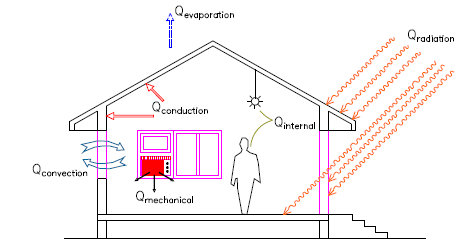
\includegraphics[width=0.8\textwidth]{figures/HeatTransferProcess}
	\caption{Pertukaran kalor bangunan dengan lingkungan \cite{skripsiIchfan}}
	\label{fig:3:HeatTransferProcess}
\end{figure}

Lingkungan termal bangungan dipengaruhi oleh beberapa faktor. Faktor-faktor tersebut diantaranya geometri bangunan, material bangunan, iklim, dan penggunaan bangunan itu sendiri. Proses perpindahan kalor yang membentuk lingkungan termal secara rinci dibagi menjadi 4 bagian, yaitu:

\begin{enumerate}
	\item Proses perpindahan panas yang terjadi di muka luar dari selubung bangunan
	\item Proses perpindahan panas yang terjadi di selubung bangunan
	\item Proses perpindahan panas yang terjadi di muka dalam dari selubung bangunan
	\item Proses perpindahan panas dan massa yang terjadi di udara dalam bangunan
\end{enumerate}

%\noindent Keempat proses perpindahan kalor ini diringkas pada Gambar \ref{fig:3:HeatTransferScheme}.

%\begin{figure}[!h]
%	\centering
%	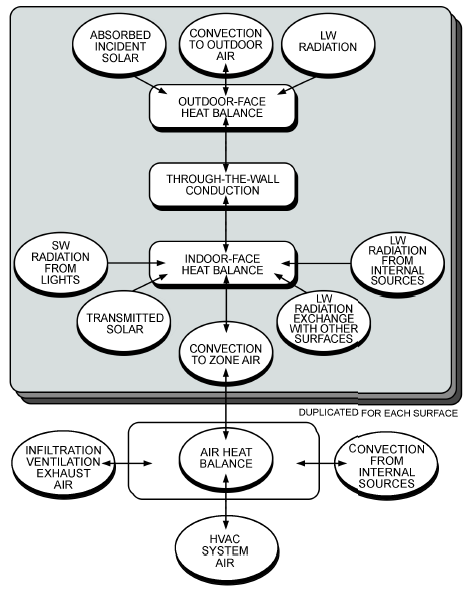
\includegraphics[width=0.8\textwidth]{figures/HeatTransferScheme}
%	\caption{Skema keseimbangan proses perpindahan panas dalam bangunan\cite{skripsiIchfan}}
%	\label{fig:3:HeatTransferScheme}
%\end{figure}

%\subsection{Kenyamanan Termal}
%Kenyamanan termal adalah suatu kondisi pikiran yang mengekspresikan kepuasan dengan lingkungan termal, baik secara fisiologis maupun psikologis, dan dinilai dengan evaluasi subyektif oleh penghuni itu sendiri \cite{ASHRAE55}. Kenyamanan termal penting untuk kesehatan dan kebugaran tubuh manusia. Hal tersebut berpengaruh terhadap produktivitas manusia dalam melakukan kegiatan. Kurangnya kenyamanan termal dapat mengakibatkan kondisi stres bagi penghuni bangunan. Apabila kondisi bangungan terlalu panas, maka penghuni akan merasa lelah. Apabila kondisi bangunan terlalu dingin, maka penghuni akan merasa gelisah dan bimbang. Dalam hal sensasi, kenyamanan termal digambarkan sebagai sensasi termal dalam bentuk \textit{too warm} atau \textit{too cold}, yang ditentukan oleh skala tujuh poin sensasi termal berdasarkan ASHRAE sebagai berikut:

%\qquad\qquad\qquad\qquad\qquad\qquad -3 = cold

%\qquad\qquad\qquad\qquad\qquad\qquad -2 = cool

%\qquad\qquad\qquad\qquad\qquad\qquad -1 = slightly cool

%\qquad\qquad\qquad\qquad\qquad\qquad\ 0 = neutral

%\qquad\qquad\qquad\qquad\qquad\qquad\ 1 = slightly warm

%\qquad\qquad\qquad\qquad\qquad\qquad\ 2 = warm

%\qquad\qquad\qquad\qquad\qquad\qquad\ 3 = hot


%Standar SNI terkait kenyamanan termal ruangan, yaitu menjaga suhu dan kelembapan ruangan pada nilai tertentu. Nilai standar suhu ruang (\textit{drybulb}) dijaga pada nilai $25\pm 1^{\circ}C$, dan nilai kelembapan dalam bentuk \textit{relative humidity} (RH), dijaga pada nilai $60\% \pm 10\%$ untuk kenyamanan penghuni \cite{SNI-03-06390-2000}.

\section{Kontrol Otomatis}

Kontrol otomatis telah memegang peranan yang sangat penting dalam perkembangan ilmu dan teknologi. Di samping sangat diperlukan pada pesawat ruang angkasa, peluru kendali, sistem kontrol pesawat, dan sebagainya, sistem kontrol juga mejadi bagian penting dan terpadu dari proses-proses dalam pabrik dan industri modern. Sistem kontrol otomatis sangat diperlukan dalam operasi-operasi di industri untuk mengendalikan tekanan, temperatur, laju aliran dan sebagainya. \cite{ControlSystemBook}

\subsection{Dasar-dasar Ilmu Kontrol}

Sistem adalah kombinasi dari beberapa komponen yang bekerja bersama-sama dan bersinergi untuk mencapai tujuan yang diinginkan. Sistem tidak dibatasi hanya untuk sistem fisik saja. Konsep sistem dapat digunakan pada gejala yang abstrak dan dinamis lainnya seperti sistem ekonomi, biologi, organisasi, dan lain sebagainya. Sistem kontrol adalah interkoneksi dari berbagai komponen kontrol yang membentuk suatu konfigurasi sistem yang akan menghasilkan respon sistem yang diinginkan. \cite{ControlSystemBook}

Komponen utama dari sistem kontrol terdiri dari proses dan kontroler. Proses adalah komponen atau grup yang terdiri dari beberapa komponen yang dikendalikan. Kontroler adalah komponen yang mengendalikan proses. Keluaran dari kontroler adalah nilai variabel yang memanipulasi proses.

Sistem kontrol dapat dikategorikan menjadi dua macam, yakni sistem kontrol kalang terbuka dan sistem kontrol kalang tertutup. Sistem kontrol kalang terbuka adalah sistem kontrol yang keluarannya tidak berpengaruh pada aksi kontrol. Pada sistem ini keluaran tidak dibandingkan dengan \textit{set point}. Dengan demikian, setiap \textit{setpoint} memiliki suatu kondisi operasi yang tetap. Jadi ketelitian sistem tergantung dari kalibrasi sistem. Sistem kontrol kalang terbuka ini juga tidak akan mampu bekerja jika ada gangguan internal maupun eksternal pada sistem. Sistem kontrol kalang tertutup atau sistem kontrol berumpan balik adalah sistem kontrol yang sinyal keluarannya mempunyai pengaruh langsung pada aksi kontrol. Sinyal kesalahan penggerak, yang merupakan selisih antara nilai keluaran sistem dan nilai \textit{set point} diumpankan ke kontroler untuk memperkecil kesalahan dan membuat agar nilai keluaran sistem mendekati harga yang diinginkan (\textit{set point}). Penggunaan umpan balik membuat respon sistem menjadi kurang peka terhadap gangguan internal maupun eksternal. Dengan demikian, jika dibandingkan dengan sistem kontrol kalang terbuka, sangat mungkin diperoleh sistem kontrol yang lebih teliti meskipun menggunakan komponen-komponen yang relatif kurang teliti. \cite{ControlSystemBook}

Sistem kontrol merupakan hal yang dinamis. Sistem akan memberikan respon terhadap input yang diberikan, di mana pada awalnya sistem akan memberikan suatu respon transien yang selanjutnya tercapai kondisi keadaan-ajeg yang akan mengikuti input yang diberikan. Terdapat tiga hal utama tujuan desain dan analisis dari sistem kontrol, yaitu: \cite{ControlSystemBook}
\begin{enumerate}
	\item Menghasilkan spesifikasi dari respon transien yang diinginkan.
	\item Mengurangi kesalahan pada keadaan-ajeg.
	\item Mencapai kestabilan sistem.
\end{enumerate}

\noindent \textbf{Respon Transien}

Jika suatu sistem kontrol dikenakan suatu input tertentu, sistem tidak dapat langsung mengikuti input yang diberikan, tetapi sistem terlebih dahulu akan berusaha untuk menyesuaikan karakter naturalnya dengan input yang diberikan. Respon inilah yang dinamakan respon transien dan menjadi hal penting untuk dianalisis dalam desain sistem kontrol. Sebagai contoh adalah respon sistem kontrol posisi elevator. Jika respon transien terlalu lambat maka akan membuat penumpang tidak sabar. Tetapi jika respon transien terlalu cepat maka akan membuat penumpang merasa tidak nyaman. Respon transien juga penting untuk alasan struktur. Respon transien yang terlalu cepat dapat juga menyebabkan kerusakan fisik pada peralatan yang dikendalikan.\cite{ControlSystemBook} \\

\noindent \textbf{Kestabilan Sistem}

Respon dari sistem merupakan hasil penjumlahan dari respon natural sistem dan respon paksaan. Respon natural merupakan respon sistem karena karakter natural dari sistem. Respon paksaan adalah respon sistem terhadap input atau paksaan yang diberikan pada sistem.
Sistem kontrol dikatakan stabil jika respon natural:
\begin{enumerate}
	\item pada rentang tertentu bernilai mendekati nol, sehingga keseluruhan respon hanya menyisakan respon paksaan, atau
	\item berosilasi.
\end{enumerate}

Jika respon natural dari sistem membesar sehingga lebih besar dari respon paksaannya, maka sistem dikatakan tidak stabil. Hal ini bisa mengakibatkan kondisi-kondisi yang tidak menguntungkan. Misalnya, suatu elevator akan meluncur sampai menembus atap, posisi antena akan terus berputar dan sebagainya.\\

\noindent\textbf{Proses Pengendalian}

Proses pengendalian merupakan tugas seorang insinyur kontrol untuk menganalisis sistem yang ada, dan merancang sistem baru untuk memenuhi kebutuhan spesifik. Terkadang sistem baru perlu dirancang, tetapi suatu unit kontroler lebih sering dirancang untuk meningkatkan kinerja sistem yang ada. Ketika perancangan suatu sistem atau penerapan suatu kontroler dalam menambah sistem yang ada, perlu mengikuti beberapa langkah berikut: \cite{ControlSystemBook}
\begin{enumerate}
	\item Pemodelan sistem
	\item Analisis sistem
	\item Perancangan kontroler
	\item Penerapan kontroler dan pengujian
\end{enumerate}

\subsection{\textit{Steady-State Error}}

Salah satu tujuan dari desain dan analisis dari sistem kontrol difokuskan pada respon keadaan-ajeg. Misalnya dalam sistem kontrol posisi elevator, kesalahan pada keadaan-ajeg akan menyebabkan posisi elevator tidak tepat pada lantai yang dituju, tetapi mungkin pada posisi di atas atau di bawahnya. Dalam keadaan-ajeg diharapkan respon sistem sesuai dengan input yang diberikan. Tujuan dari desain dan analisis sistem kontrol diarahkan pada bagaimana memperkecil kesalahan pada keadaan-ajeg.

kesalahan keadaan-ajeg (\textit{steady-state error}) adalah perbedaan antara input dan output untuk input tes yang ditentukan ketika $t \rightarrow \infty$. Dalam sistem kontrol diperhatikan perbedaan antara input dan output dari sistem kontrol umpan balik setelah mencapai keadaan-ajeg. \cite{ControlSystemBook}

%Dengan demikian, hal ini dibatasi untuk sistem yang stabil, dimana respons alami mendekati nol selayaknya $t \rightarrow \infty$ . Sistem yang tidak stabil merepresentasikan hilangnya kendali dalam keadaan-ajeg dan sama sekali tidak dapat diterima untuk digunakan. Persamaan yang diperoleh untuk menghitung galat keadaan-ajeg dapat diterapkan secara keliru ke sistem yang tidak stabil. Dengan demikian, insinyur harus memeriksa stabilitas sistem saat melakukan analisis dan perancangan galat keadaan-ajeg.

\begin{figure}[!h]
	\centering
	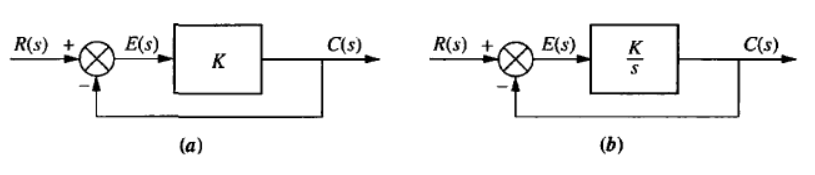
\includegraphics[width=1\textwidth]{figures/SSEExample}
	\caption{Sistem dengan \textbf{a.} \textit{steady-state error} bernilai terbatas untuk input fungsi step; \textbf{b.} \textit{steady-state error} nol untuk input fungsi step \cite{ControlSystemBook}}
	\label{fig:3:steadystateerror}
\end{figure}

Contohnya, amati Gambar \ref{fig:3:steadystateerror}(a) di mana $R(s)$ merupakan input, $C(s)$ merupakan output, dan $E(s) = R(s) - C(s)$ adalah galat (galat keadaan-ajeg). Pada keadaan-ajeg, jika $c(t) = r(t)$, maka $e(t)$ bernilai nol.

%Tetapi dengan adanya \textit{gain} (pengali) $K$, galat tersebut, $e(t)$, tidak dapat bernilai nol jika $c(t)$ bernilai terbatas dan tak nol. Dengan demikian, keutamaan dari konfigurasi sistem (\textit{gain} murni K pada umpan maju), haruslah memiliki nilai galat. Jika kita sebut $c_{steady-state}$ adalah nilai keadaan-ajeg suatu output dan $e_{steady-state}$ adalah nilai keadaan-ajeg suatu galat, maka $c_{steady-state} = K e_{steady-state}$, atau 

%\begin{equation} \label{eq:3:steady-state-error}
%e_{steady-state} = \frac{1}{K} \ c_{steady-state}
%\end{equation}

%Dengan demikian, semakin besar nilai K dan semakin kecil nilai $e_{steady-state}$ haruslah menghasilkan nilai $c_{steady-state}$ yang sama. Kesimpulan yang dapat ditarik yaitu \textit{gain} murni pada umpan maju akan selalu menimbulkan suatu galat keadaan-ajeg untuk input fungsi step. galat ini berkurang ketika nilai K meningkat.

%Jika penguatan jalur maju digantikan oleh integrator, seperti yang ditunjukkan pada Gambar \ref{fig:3:steadystateerror}(b), akan ada nol galat pada kondisi ajeg untuk input fungsi steo. Alasannya adalah sebagai berikut: Ketika $c(t$ meningkat, $e(t)$ akan berkurang, karena $e(t) = r(t) - c(t)$. Penurunan ini akan berlanjut hingga tidak ada galat nol, tetapi masih akan ada nilai untuk $c(t)$ karena integrator dapat memiliki output yang konstan tanpa input apa pun. Misalnya, motor dapat direpresentasikan hanya sebagai integrator. Tegangan yang diberikan pada motor akan menyebabkan putaran. Ketika tegangan yang diberikan dilepas, motor akan berhenti dan tetap pada posisi keluaran saat ini. Karena tidak kembali ke posisi semula, kami memiliki output perpindahan sudut tanpa input ke motor. Oleh karena itu, sistem yang mirip dengan Gambar \ref{fig:3:steadystateerror}(b), yang menggunakan motor di jalur maju, dapat memiliki nol kondisi ajeg untuk input fungsi step \cite{ControlSystemBook}.

%\begin{figure}[!h]
%	\centering
%	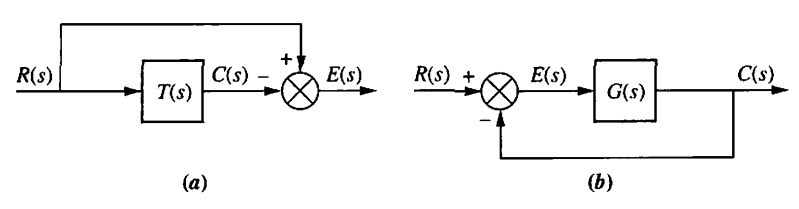
\includegraphics[width=0.75\textwidth]{figures/SSEExample2}
%	\caption{Galat sistem kontrol tertutup: a. Representasi secara umum; b. Representasi untuk sistem umpan balik satuan}
%	\label{fig:3:steadystateerror2}
%\end{figure}

%Pertimbangkan Gambar \ref{fig:3:steadystateerror2}(a). Untuk menentukan $E(s)$, galat antara input, $R(s)$, dan output, $C(s)$, ditulis sebagai:
%\begin{equation} \label{eq:3:steady-state-error2}
%E(s) = R(s) - C(s)
%\end{equation}
%tetapi,
%\begin{equation} \label{eq:3:steady-state-error3}
%C(s) = R(s)T(s)
%\end{equation}
%Dengan mensubstitusi Persamaan \ref{eq:3:steady-state-error3} ke \ref{eq:3:steady-state-error2}, lalu disederhanakan dan dicari solusi pemecahan untuk $E(s)$, yaitu:
%\begin{equation} \label{eq:3:steady-state-error4}
%E(s) = R(s)(1 - T(s))
%\end{equation}
%Meskipun Persamaan \ref{eq:3:steady-state-error4} membantu kita dalam menyelesaikan $e(t)$ di setiap waktu, t, tetapi kita lebih tertarik untuk mengetahui nilai akhir dari galat, $e(\infty)$. Dengan mengaplikasikan teorema nilai akhir, yang mana memungkinkan kita untuk menggunakan nilai akhir dari $e(t)$ tanpa mengambil transformasi balik Laplace $E(S)$, dan kemudian membiarkan $t$ mendekati $\infty$, didapatkan
%\begin{equation} \label{eq:3:steady-state-error5}
%e(\infty) = \lim_{t \to \infty} e(t) = \lim_{s \to 0} sE(s)
%\end{equation}
%Substitusi Persamaan \ref{eq:3:steady-state-error4} ke \ref{eq:3:steady-state-error5}, didapatkan:
%\begin{equation} \label{eq:3:final-steady-state-error}
%e(\infty) = \lim_{t \to \infty} e(t) = \lim_{s \to 0} sR(s)[1 - T(s)]
%\end{equation}

%Pertimbangkan sistem kontrol umpan balik ditunjukkan pada Gambar \ref{fig:3:steadystateerror2}(b). Karena umpan balik, $H(s)$, sama dengan 1, sistem memiliki umpan balik satuan. Implikasinya adalah bahwa $E(s)$ sebenarnya adalah galat antara input, $R(s)$, dan output, $C(s)$. Jadi, jika kita memecahkan Persamaan untuk $E(s)$, kita akan memiliki ekspresi untuk galat tersebut. Kemudian diterapkan teorema nilai akhir untuk mengevaluasi galat keadaan-ajeg.

%Menulis $E(s)$ berdasarkan Gambar \ref{fig:3:steadystateerror2}(b), didapatkan
%\begin{equation} \label{eq:3:sse-g}
%E(s) = R(s) - C(s)
%\end{equation}
%Tetapi,
%\begin{equation} \label{eq:3:sse-g2}
%C(s) = E(s)G(s)
%\end{equation}
%Substitusi Persamaan \ref{eq:3:sse-g2} ke \ref{eq:3:sse-g}, didapatkan:
%\begin{equation} \label{eq:3:sse-g3}
%E(s) = \frac{ R(s) }{ 1 + %G(s) }
%\end{equation}
%Kemudikan diterapkan teorema nilai akhir, \ref{eq:3:steady-state-error5}. Pada titik ini dalam perhitungan numerik, kita harus memeriksa apakah sistem loop tertutup stabil, menggunakan, misalnya, kriteria Routh-Hurwitz. Namun, untuk saat ini, asumsikan bahwa sistem loop tertutup adalah stabil dan gantikan Persamaan \ref{eq:3:sse-g3} ke Persamaan \ref{eq:3:steady-state-error5}, didapatkan:
%\begin{equation} \label{eq:3:sse-g4}
%e(\infty) = \lim_{s \to 0} \frac{ sR(s) }{ 1 + G(s) }
%\end{equation}


\section{Jaringan Saraf Tiruan (JST)}
Jaringan Saraf Tiruan (JST) dimodelkan dengan mengadaptasi proses biologis untuk pemrosesan informasi, termasuk secara khusus sistem saraf dan unit dasarnya, neuron (sel saraf). Sinyal didistribusikan dalam bentuk beda potensial antara bagian dalam dan luar sel. Komponen sel saraf (neuron) ditunjukkan pada Gambar \ref{fig:3:neuron}. Dendrit membawa sinyal dari neuron lain ke dalam badan sel (soma), kemungkinan dengan memperkalikan setiap sinyal yang masuk dengan koefisien pembobotan pengiriman. \cite{NNControlBook}

\begin{figure}[!h]
	\centering
	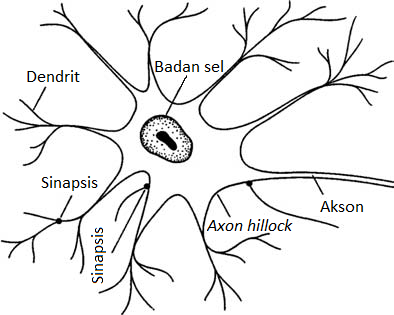
\includegraphics[width=0.5\textwidth]{figures/neuron}
	\caption{Anatomi neuron \cite{NNControlBook}}
	\label{fig:3:neuron}
\end{figure}

Pada badan sel, kapasitansi sel mengintegrasikan sinyal yang terkumpul di \textit{axon hillock} (bagian khusus dari badan sel neuron yang terhubung dengan akson). Sekalinya sinyal gabungan melebihi ambang batas nilai tertentu, sinyal/impuls ditransmisikan melalui akson. Ketidaklinieran sel menjadikan impuls komposit sebagai fungsi nonlinier dari kombinasi sinyal yang datang. Akson tersebut, melalui sinapsis, terhubung dengan dendrit pada neuron berikutnya. Sinapsis beroperasi melalui pelepasan kimiawi \textit{neurotransmitter} melintasi celah antar sel, dan dapat berupa \textit{excitatory} (kecenderungan dalam pengaktifan neuron berikutnya) atau \textit{inhibitory} (kecenderungan dalam mencegah pengaktifan neuron berikutnya) \cite{NNControlBook}.

\subsection{Model Matematis Neuron}

Model matematis dari suatu neuron dilukiskan oleh Gambar \ref{fig:3:math}, yang mana menunjukkan pembobotan dendrit $v_j$, nilai ambang batas $v_0$ (disebut juga sebagai bias), penjumlahan dari sinyal masuk yang diberi bobot, dan fungsi nonlinear $\sigma(\cdot)$. Sel input adalah sinyal ke-$n$ pada waktu instan 	$kx_1(k), kx_2(k), kx_3(k),...,x_n(k)$ dan outputnya adalah nilai skalar $y(k)$, yang dapat dinyatakan sebagai

\begin{figure}[!h]
	\centering
	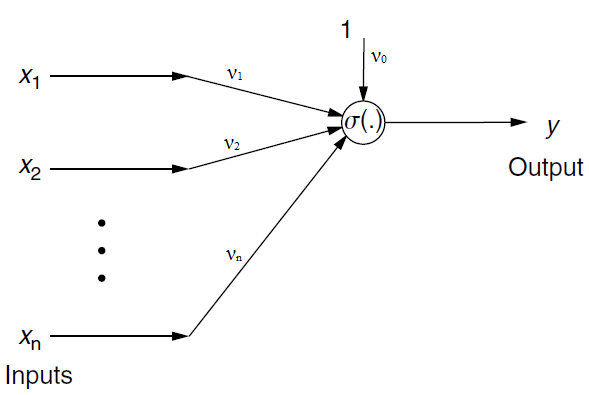
\includegraphics[width=0.5\textwidth]{figures/neuronmath}
	\caption{Model matematis neuron \cite{NNControlBook}}
	\label{fig:3:math}
\end{figure}

\begin{equation} \label{eq:3:perceptron}
y(k) = \sigma \left( \sum_{j=1}^{n}v_jx_j(k)+v_0 \right)
\end{equation}

Bobot-bobot positif  $v_j$ berhubungan dengan sinapsis \textit{exitatory} dan bobot-bobot negatif dengan sinapsis \textit{inhibitory}. Jaringan ini disebut sebagai \textit{perceptron} oleh Rosenblatt pada tahun 1959. \cite{NNControlBook}

Fungsi sel nonlinear dikenal sebagai fungsi aktivasi. Fungsi aktivasi dipilih secara khusus untuk aplikasi-aplikasi meskipun beberapa pilihan yg umum diilustrasikan pada Gambar \ref{fig:3:activation}. Intensi pada fungsi aktivasi adalah untuk memodelkan perilaku nonlinier suatu sel di mana tidak terdapat output di bawah nilai tertentu suatu argumen. Fungsi sigmoid adalah sebuah kelas umum dari fungsi yang tidak meningkat secara monoton dengan mengambil nilai-nilai yang dibatasi antara nilai $-\infty$ dan $+\infty$. 
\begin{figure}[!h]
	\centering
	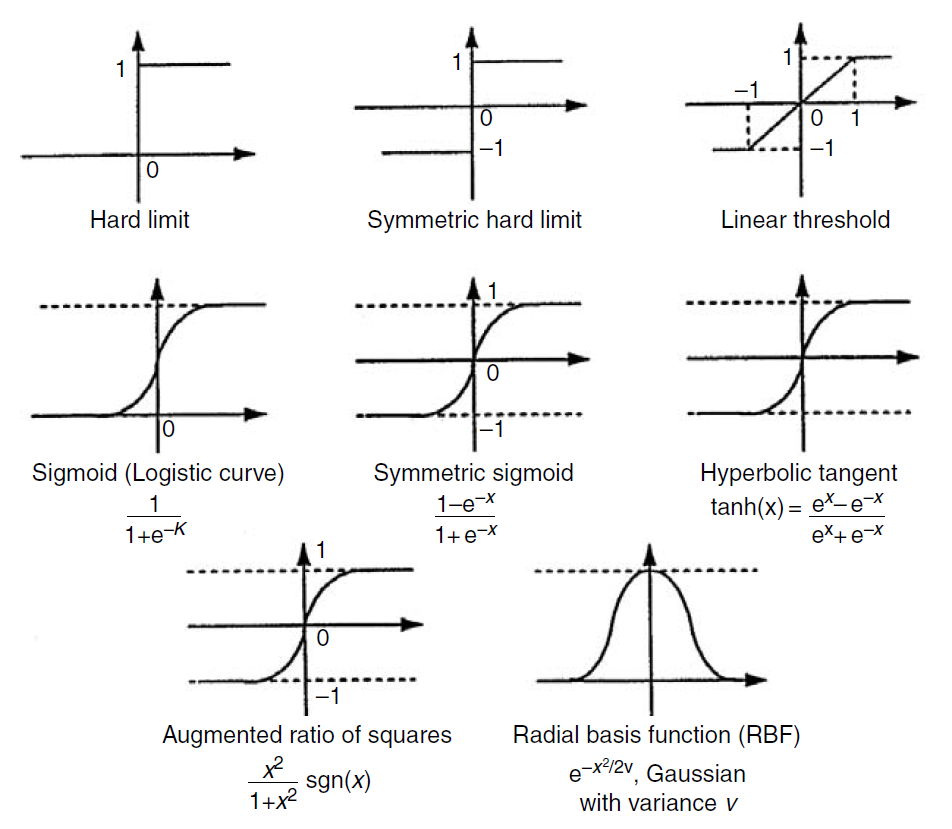
\includegraphics[width=0.6\textwidth]{figures/activationFunction}
	\caption{Fungsi-fungsi aktivasi \cite{NNControlBook}}
	\label{fig:3:activation}
\end{figure}
Perlu dicatat bahwa ketika nilai ambang batas atau bias $v_0$ berubah, fungsi aktivasi bergeser ke kiri atau ke kanan. Untuk kebanyakan algoritma pelatihan JST (termasuk \textit{backpropagation}), turunan dari $\sigma(\cdot)$ dibutuhkan sehingga fungsi aktivasi yang dipilih haruslah dapat terdiferensiasi. \cite{NNControlBook}

Ekspresi untuk output neuron $y(k)$ pada waktu instan $k$ (dalam kasus waktu yang kontinyu) dapat dirampingkan dengan menentukan vektor kolom dari bobot-bobot JST $\ \overline{v}(k) \in \mathbb{R}^n $ sebagai
\vspace{-1em}
\begin{equation} \label{eq:3:vektorKolom}
\overline{x}(k) = [x_1\ x_2\ \cdots\ x_n]^T, \qquad \overline{v}(k) = [v_1\ v_2\ \cdots\ v_n]^T
\end{equation}

Kemudian, ini memungkinkan untuk ditulis dalam notasi matriks
\vspace{-1em}
\begin{equation} \label{eq:3:matriksy}
y = \sigma(\overline{v}^T\overline{x}) + v_0
\end{equation}

Vektor kolom input \textit{augmented} $x(k) \in \mathbb{R}^{n+1} $ dan vektor kolom bobot JST $v(k) \in \mathbb{R}^{n+1} $ didefinisikan sebagai
\vspace{-1em}
\begin{equation} \label{eq:3:matriksaugmented}
\begin{split}
x(k) = [1\;\; \overline{x}^T]^T = [1\;\; x_1\ x_2\ \cdots\ x_n]^T \\
v(k) = [v_0\ \overline{v}^T]^T = [v_0\ v_1\ v_2\ \cdots\ v_n]^T
\end{split}
\end{equation}

yang dapat juga ditulis sebagai
\vspace{-2em}
\begin{equation} \label{eq:3:matriksfinal}
\begin{split}
y = \sigma(v^Tx)
\end{split}
\end{equation}

\begin{figure}[!h]
	\centering
	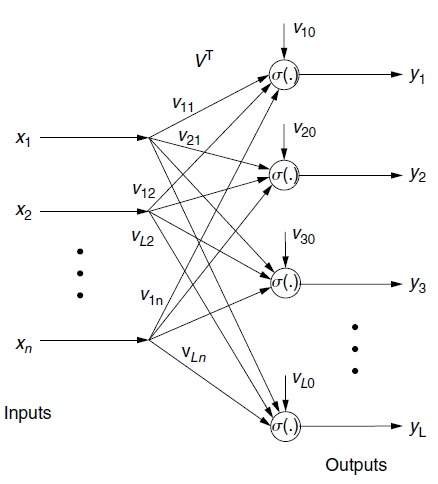
\includegraphics[width=0.5\textwidth]{figures/jstTunggal}
	\caption{Jaringan layar tunggal \cite{NNControlBook}}
	\label{fig:3:jstTunggal}
\end{figure}
Meskipun vektor input $\overline{x}(k) \in \mathbb{R}^n $ dan vektor bobot $\overline{v}(k) \in \mathbb{R}^n $ masing-masing telah ditambahkan dengan 1 dan $v_0$, untuk memasukkan nilai bias, terkadang dengan bebas dapat dinyatakan bahwa $x(k)$ dan $v$ adalah elemen $\mathbb{R}^n$.

Vektor penggambaran output neuron $y(k)$ disebut sebagai mekanisme penarikan sel. Vektor tersebut mendeskripsikan bagaimana output itu direkonstruksi dari sinyal input dan nilai parameter sel.

Gambar \ref{fig:3:jstTunggal} menunjukkan sebuah JST yang mengandung L buah sel, semuanya diberi umpan oleh sinyal input yang sama dan memproduksi satu output $y(k)$ per neuron. Hal ini disebut sebagai jaringan layar tunggal. Persamaan \textit{recall} untuk jaringan ini ditunjukkan sebagai berikut
\vspace{0em}
\begin{equation} \label{eq:3:recall}
y_l(k) = \sigma \left( \sum_{j=1}^{n}v_{lj}x_j(k)+v_{l0} \right); \qquad l = 1,2,...,L
\end{equation}

Akan lebih mudah untuk menulis bobot dan bias masing-masing dalam bentuk matriks dan vektor. Dengan menentukan matriks bobot dan vektor bias sebagai berikut
\vspace{-1em}
\begin{equation} \label{eq:3:weightVector}
\overline{V}^T \equiv
\left[
\begin{matrix}
v_{11} & v_{12} & \cdots & v_{1n} \\
v_{21} & v_{22} & \cdots & v_{2n} \\
\vdots & \vdots & \ddots & \vdots \\
v_{L1} & v_{L2} & \cdots & v_{Ln} \\
\end{matrix}
\right], \qquad
b_v = 
\left[
\begin{matrix}
v_{10} \\
v_{20} \\
\vdots \\
v_{L0} \\
\end{matrix}
\right],
\end{equation}

\noindent Salah satu cara menulis vektor output $y(t) = [y_0\ y_1\ y_2\ \cdots y_L]^T$ sebagai berikut
\vspace{-1em}
\begin{equation} \label{eq:3:outputVector}
y = \overline{\sigma}(\overline{V}^T\overline{x}+b_v)
\end{equation}
\noindent Vektor fungsi aktivasi yang ditentukan oleh vektor $w\equiv [w_1\ w_2\ \cdots w_L]^T$ adalah
\vspace{-1em}
\begin{equation} \label{eq:3:activation}
\overline{\sigma}(w)\equiv [\overline{\sigma}(w)_1\ \overline{\sigma}(w)_2\ \cdots\ \overline{\sigma}(w)_L]^T
\end{equation}

Penyempurnaan lebih lanjut dapat dicapai dengan memasukkan vektor bias sebagai kolom pertama dari matriks \textit{augmented} bobot sebagai berikut
\vspace{-1em}
\begin{equation} \label{eq:3:fullVector}
V^T \equiv
\left[
\begin{matrix}
v_{10} & v_{11} & \cdots & v_{1n} \\
v_{20} & v_{21} & \cdots & v_{2n} \\
\vdots & \vdots & \ddots & \vdots \\
v_{L0} & v_{L1} & \cdots & v_{Ln} \\
\end{matrix}
\right]
\end{equation}\

Kemudian output JST dapat digambarkan dalam bentuk vektor \textit{augmented} input $x(k)$ sebagai
\vspace{0em}
\begin{equation} \label{eq:3:finalVector}
y = \overline{\sigma}(V^Tx)
\end{equation}

\subsection{Jaringan Layar Jamak (MLP)}
Jaringan layar jamak (\textit{Multilayer Perceptron}) merupakan perluasan dari jaringan layar tunggal (\textit{perceptron}). Sebuah JST 2 layar memiliki dua lapisan neuron dengan satu layar memiliki $L$ buah neuron yang memberikan umpan kepada lapisan kedua yang memiliki $m$ buah neuron, digambarkan pada Gambar \ref{fig:3:mlp}. Lapisan pertama dikenal sebagai lapisan tersembunyi, dengan $L$ sebagai jumlah neuron pada lapisan tersembunyi tersebut. Lapisan kedua dikenal sebagai lapisan output. Jaringan saraf tiruan yang terdiri dari banyak lapisan disebut sebagai \textit{multilayer perceptron}. Daya komputasi untuk lapisan ini perlu ditingkatkan secara signifikan dibandingkan jaringan layar tunggal. Dengan jaringan layar tunggal, dimungkinkan untuk menerapkan operasi digital seperti AND, OR, dan COMPLEMENT. 
\begin{figure}[!h]
	\centering
	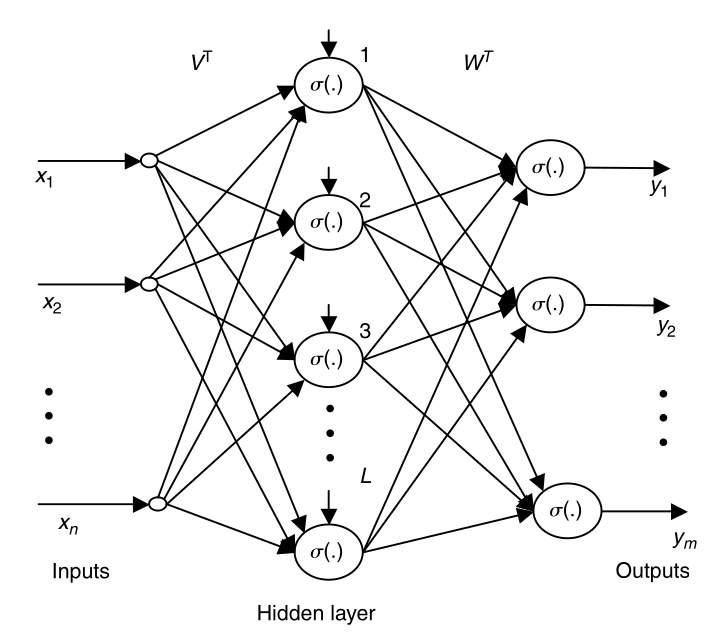
\includegraphics[width=0.65\textwidth]{figures/mlp}
	\caption{Jaringan 2 layar \cite{NNControlBook}}
	\label{fig:3:mlp}
\end{figure}
Namun, penelitian mengenai JST telah dihentikan bertahun-tahun yang lalu ketika ditunjukkan bahwa jaringan layar tunggal tidak mampu melakukan operasi EXCLUSIVE OR (X-OR), yang merupakan masalah dasar dalam perancangan sistem logika digital. Kemudian telah ditunjukkan bahwa jaringan 2 layar dapat menerapkan operasi EXCLUSIVE OR (X-OR) dan ini kembali mempercepat penelitian JST di awal 1980-an. Beberapa peneliti (Hush dan Horne 1993) mempresentasikan solusi untuk operasi X-OR dengan menggunakan fungsi aktivasi sigmoid. \cite{NNControlBook}

\noindent Output jaringan 2 layar ditunjukkan oleh persamaan \textit{recall} berikut
\begin{equation} \label{eq:3:2layerOut}
y_i = \sigma
\left(
\sum_{l=1}^{L}w_{il}\sigma
	\left(
		\sum_{j=1}^{n}v_{lj}x_j + v_{l0}
	\right)
	+ w_{i0}
\right); \qquad i = 1,2,\dots,m
\end{equation}
\vspace{1em}

\noindent Definisi output jaringan tersembunyi $z_1$ dapat ditulis sebagai berikut
\begin{equation} \label{eq:3:hiddenlayer}
\begin{split}
z_l = \sigma\left(\sum_{j=1}^{n}v_{lj}x_j+v_{l0} \right);\qquad l = 1,2,\dots,L\\
y_i = \sigma\left(\sum_{l=1}^{L}w_{il}z_l+w_{i0} \right);\qquad l = 1,2,\dots,m
\end{split}
\end{equation}
\vspace{1em}

\noindent Definisi matriks bobot layar pertama $\overline{V}$ dan $V$ dan matriks bobot layar kedua sebagai berikut
\begin{equation} \label{eq:3:weight21Vector}
\overline{W}^T \equiv
\left[
\begin{matrix}
w_{11} & w_{12} & \cdots & w_{1n} \\
w_{21} & w_{22} & \cdots & w_{2n} \\
\vdots & \vdots & \ddots & \vdots \\
w_{L1} & w_{L2} & \cdots & w_{Ln} \\
\end{matrix}
\right], \qquad
b_w = 
\left[
\begin{matrix}
w_{10} \\
w_{20} \\
\vdots \\
w_{L0} \\
\end{matrix}
\right],
\end{equation}
\begin{equation} \label{eq:3:weight22Vector}
W^T \equiv
\left[
\begin{matrix}
w_{10} & w_{11} & \cdots & w_{1n} \\
w_{20} & w_{21} & \cdots & w_{2n} \\
\vdots & \vdots & \ddots & \vdots \\
w_{L0} & w_{L1} & \cdots & w_{Ln} \\
\end{matrix}
\right]
\end{equation}

\noindent Output JST dapat ditulis sebagai berikut
\begin{equation} \label{eq:3:2layer}
y = \overline{\sigma}
\left(
	\overline{W}^T\overline{\sigma}(\overline{V}^T\overline{x}+b_v)+b_w
\right),
\end{equation}
atau
\begin{equation} \label{eq:3:2layerfinal}
y = \overline{\sigma}
\left(
	W^T\sigma(V^Tx)
\right).
\end{equation}
Pada Persamaan \ref{eq:3:2layerfinal}, notasi $\overline{\sigma}$ berarti bahwa vektor ditentukan sesuai dengan Persamaan (\ref{eq:3:activation}). Dalam Persamaan (\ref{eq:3:2layerfinal}) perlu digunakan vektor \textit{augmented}
\begin{equation} \label{eq:3:augVector}
\sigma(w) \equiv [1\quad \overline{\sigma}(w)^T]^T = [1\quad \sigma(w_1)\ \sigma(w_2)\ \dots\ \sigma(w_L)\ ]^T,
\end{equation}
\noindent di mana nilai 1 ditempatkan sebagai entri pertama untuk memungkinkan penggabungan bias $w_{i0}$ sebagai kolom pertama dari $W^T$. Dalam hal vektor output layar tersembunyi $z\in \mathbb{R}^L$ seseorang dapat menuliskan
\begin{equation} \label{eq:3:final19}
\overline{z} = \sigma(V^Tx),
\end{equation}
\begin{equation} \label{eq:3:final20}
y = \sigma(W^Tz).
\end{equation}
\noindent di mana $z \equiv [1\quad \overline{z}^T]^T$

\subsubsection{Penskalaan Fitur}

Salah satu transformasi terpenting yang perlu diterapkan pada data sebelum pelatihan model JST adalah penskalaan fitur. Dengan sedikit pengecualian, algoritma JST tidak berfungsi dengan baik saat atribut numerik masukan memiliki skala yang sangat berbeda. Akan tetapi, harus diperhatikan bahwa penskalaan nilai data target umumnya tidak diperlukan. Ada dua cara umum untuk membuat semua atribut memiliki skala yang sama, yaitu dengan metode \textit{Min-Max Scaling} dan metode \textit{Standardization} \cite{HandsOnML}. Pada penelitian ini hanya digunakan penskalaan fitur metode \textit{Min-Max Sclaing}. Penskalaan min-maks (\textit{Min-Max Scaling}) bertujuan untuk meningkatkan kinerja JST menjadi optimal dengan menyamakan rentang nilai dan besar satuan dari setiap variabel (berupa rentang nilai dari 0 hingga 1). Masing-masing variabel diubah menjadi skala satuan dengan melakukan transformasi data secara statistik. Data dari setiap variabel akan dikurangi dengan nilai minimum variabel tersebut yang dikemudian dibagi oleh selisih dari nilai maksimum dan nilai minimum variabel tersebut. Secara lengkap dapat dituliskan pada Persamaan \ref{eq:3:MinMaxScaler}.

\begin{equation} \label{eq:3:MinMaxScaler}
z = \frac{x_i - min(x)}{max(x) - min(x)}
\end{equation}

\subsubsection{Evaluasi Kinerja Model JST}

Dalam mengevaluasi model JST untuk permasalahan regresi terdapat beberapa evaluasi kinerja seperti \textit{mean absolute error} (MAE) dan \textit{mean squared error} (MSE). Perhitungan evaluasi kinerja tersebut didefinisikan sebagai berikut:

\begin{equation} \label{eq:3:MAEequation}
	MAE = \frac{1}{m} \sum_{i=1}^{m} |y^i-T^i|
\end{equation}

\begin{equation} \label{eq:3:MSEequation}
	MSE = \frac{1}{m} \sum_{i=1}^{m} (y^i-T^i)^2
\end{equation}

\noindent di mana:\\
$y$ = nilai prediksi model\\
$T$ = nilai data target

Pada umumnya, MSE digunakan untuk mengevaluasi kinerja arsitektur model JST. Nilai MSE jauh lebih sensitif dibandingkan nilai MAE dalam menunjukan galat prediksi model. Hal itu dikarenakan MSE mampu menunjukkan galat yang diakibatkan oleh adanya penyimpangan (standar deviasi) dan akibat adanya data \textit{outliers}. Dengan demikian, MSE biasa digunakan dalam proses pelatihan model dan penentuan rancangan model JST. Kemudian, MAE dapat digunakan untuk melakukan padanan galat prediksi model dengan besaran fisis aslinya. Nilai MAE dapat dijadikan tolak ukur kelayakan akhir suatu model JST. Toleransi MAE bergantung kepada besaran fisis dari variabel yang sedang diteliti. \cite{HandsOnML}

\section{Kontrol Jaringan Saraf Tiruan}

Untuk mengendalikan lingkungan termal, pada umumnya digunakan sistem kontrol modern (\textit{modern control system}). Hal ini didasarkan pada karakteristik lingkungan termal yang memiliki sifat MIMO (\textit{multiple input multiple output}). Dengan demikian, sistem kontrol klasik tidak tepat digunakan untuk sistem \textit{climate chamber}.
\begin{table}[!h]
	\caption{Perbandingan metode kontrol}
	\label{tbl:3:whyann}
	\centering
	% use packages: array
	\begin{tabular}{|p{4cm}|p{4cm}|p{4.5cm}|}
		\hline
		\textbf{Metode kontrol} & \textbf{Klasik} & \textbf{Modern} \\ 
		\hline
		Domain & Frekuensi, Domain-S & Waktu, Domain-t \\ 
		\hline
		Representasi Model & Fungsi Transfer & State-Space \\ 
		\hline
		Kontinyuitas & Kontinyu & Kontinyu, Diskrit, \textit{Hybrid} \\ 
		\hline
		Linieritas & Linier & Linier, Nonlinier \\ 
		\hline
		Variansi waktu & \textit{Time-invariant} (TI) & \textit{Time-variant} (TV) \\ 
		\hline
		Dimensi & SISO & MIMO \\ 
		\hline
		Determinisme & Deterministik & Deterministik, Stokastik \\ 
		\hline
		Optimisasi & Tidak & Ya \\ 
		\hline
		Batasan & Tidak & Ya \\ 
		\hline
		Implementasi & Murah, Mudah & Mahal, Kompleks \\ 
		\hline
	\end{tabular}
\end{table}

Pada umumnya, metode kontrol klasik menggunakan perubahan domain dinamika sistem yang digambarkan oleh Persamaan Diferensial Ordiner (PDE) untuk menghindari komplekstias dari solusi PDE domain waktu. PDE dinamika sistem diubah dari domain waktu ke dalam domain frekuensi menggunakan transformasi Fourier atau secara umum menggunakan transformasi Laplace untuk domain frekuensi bilangan kompleks (domain-s), yang ekuivalen dengan transformasi Z untuk waktu diskret. Pada metode kontrol modern, alih-alih mengubah domain lebih baik menggunakan konversi persamaan diferensial orde tinggi ke dalam persamaan orde 1 domain waktu yang disebut sebagai perasamaan keadaan. Selain itu, representasi langsung dan penanganan sistem multi-input multi-output (MIMO) diperbolehkan dengan menggunakan representasi model fungsi keadaan. \cite{MPCDissertation}

Kelemahan utama dari kontrol klasik adalah bahwa kontrol ini hanya dapat digunakan untuk mengendalikan sistem \textit{single-input single-output} (SISO), dengan persyaratan pada model sistem untuk menjadi \textit{linear time-invariant} (LTI). Metode klasik memberikan hasil yang memuaskan hanya dalam mengendalikan proses sederhana, tetapi hasil yang tidak memuaskan dalam kontrol sistem yang lebih kompleks. \cite{MPCDissertation}

Pada dasarnya ada banyak sekali metode kontrol yang merupakan bagian dari metode kontrol modern. Metode-metode tersebut dapat dikelompokkan menjadi beberapa sub kategori. Kategori-kategori tersebut digambarkan dalam bentuk gambar taksonomi pada Gambar \ref{fig:3:ControlSystemTaxonomy}. Berdasarkan taksonomi yang digambarkan pada Gambar \ref{fig:3:ControlSystemTaxonomy}, dapat dilihat bahwa Jaringan Saraf Tiruan (\textit{Neural networks}) merupakan salah satu metode kontrol modern.

\begin{figure}[!h]
	\centering
	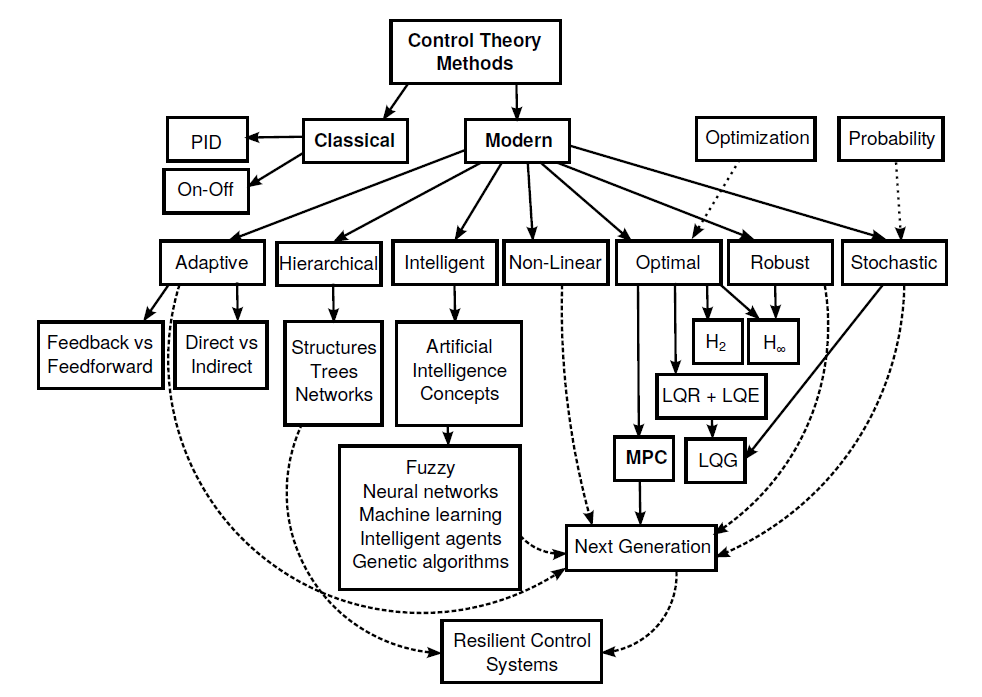
\includegraphics[width=0.8\textwidth]{figures/ControlSystemTaxonomy}
	\caption{Taksonomi metode kontrok klasik vs modern \cite{MPCDissertation}}
	\label{fig:3:ControlSystemTaxonomy}
\end{figure}
\chapter{PELAKSANAAN PENELITIAN}
\label{pelaksanaan-penelitian}

\section{Alat dan Bahan Penelitian}
Penelitian ini tidak dapat dilakukan tanpa adanya alat dan bahan yang memudahkan penulis dalam melakukan penelitian. Alat dan bahan yang digunakan oleh penulis disebutkan secara rinci pada Tabel \ref{tbl:4:alatbahan}, dan Tabel \ref{tbl:4:speklaptop}.

%\vspace{2em}
\begin{table}[!h]
	\caption{Daftar alat dan bahan}
	\label{tbl:4:alatbahan}
	\centering
	% use packages: array
	\begin{tabular}{|c|p{4.5cm}|p{9.5cm}|}
		\hline
		No. & Nama alat/bahan & Fungsi \\
		\hline
		1 & Laptop ASUS N550JX & Perangkat komputer perancangan jaringan saraf tiruan. \\
		\hline
		2 & IES-VE 2019 & Perangkat lunak untuk pengambilan data lingkungan termal \textit{climate chamber} dan variasi gangguan. \\
		\hline
		3 & MS Excel 365 & Perangkat lunak pengolahan data tabular. \\
		\hline
		4 & Visual Studio Code 1.38 & Aplikasi penulisan dan penyuntingan kode sumber. \\
		\hline
		5 & Python 3.7 & Bahasa pemrograman. \\
		\hline
		6 & Anaconda 3 & Distribusi pengelola lingkungan pengembangan dan manajemen paket untuk komputasi ilmiah. \\
		\hline
		7 & Jupyter Notebook 1.0 & Aplikasi web untuk menulis kode program, teks, persamaan, dan visualisasi. \\
		\hline
		8 & Pandas 1.0.3 & Pustaka manupulasi dan analisis data. \\
		\hline
		8 & Scikit-Learn 0.21 & Pustaka pembangunan \textit{Machine Learning}. \\
		\hline
		9 & fireTS 0.0.7 & Pustaka prediksi deret waktu multivarian. \\
		\hline
		10 & MATLAB R2016a & Perangkat lunak untuk menjalankan simulasi sistem kontrol. \\
		\hline
		%6 & Raspberry Pi versi 3 B & Komputer mikro sebagai perangkat pengendali. \\
		%\hline
	\end{tabular}
\end{table}

%\vspace{2em}
\begin{table}[!h]
	\caption{Spesifikasi laptop ASUS N550JX}
	\label{tbl:4:speklaptop}
	\centering
	% use packages: array
	\begin{tabular}{|c|p{5cm}|p{8cm}|}
		\hline
		No. & Komponen & Spesifikasi \\ 
		\hline
		1 & Processor & Intel Core i7-4720HQ CPU @ 2.60GHz x 8 \\ 
		\hline
		2 & Graphics & Intel Haswell Mobile \\
		\hline
		3 & RAM & 8 GB \\ 
		\hline
		4 & Tipe sistem operasi & 64-bit \\
		\hline
		5 & Sistem operasi I & Manjaro Linux \\ 
		\hline
		6 & Sistem operasi II & Windows 10 Home Single Language \\ 
		\hline
	\end{tabular}
\end{table}

\section{Tata Laksana Penelitian}
Alur penelitian yang digunakan penulis dalam mencapai tujuan dapat dilihat pada Gambar \ref{fig:4:TataLaksanaPenelitian} berikut.
\begin{figure}[!h]
	\centering
	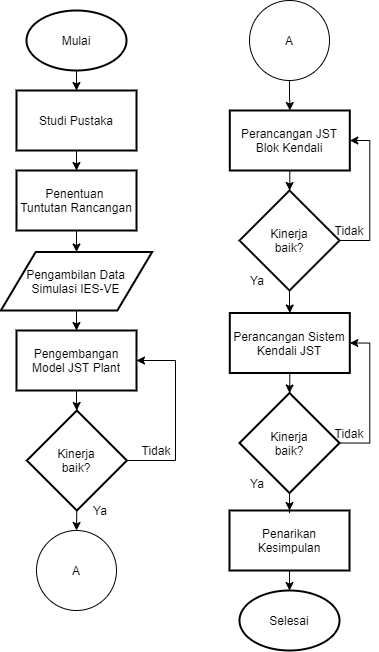
\includegraphics[width=0.3\textwidth]{figures/TataLaksanaPenelitian}
	\caption{Bagan Tata Laksana Penelitian}
	\label{fig:4:TataLaksanaPenelitian}
\end{figure}

%\begin{figure}[!h]
%	\centering
%	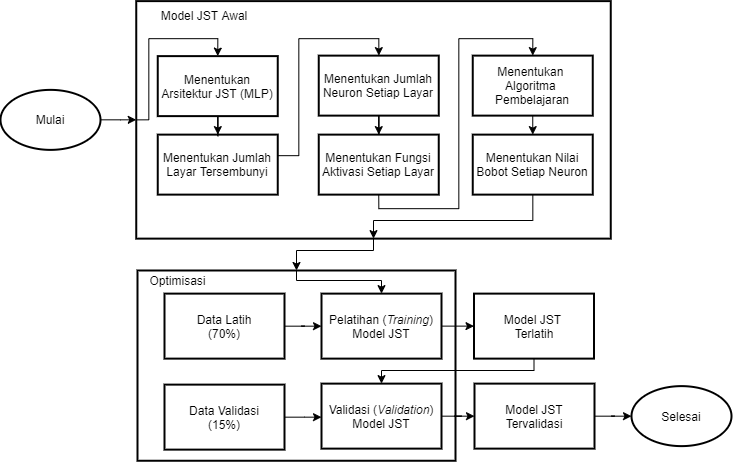
\includegraphics[width=0.85\textwidth]{figures/PerancanganModel}
%	\caption{Bagan Perancangan Model JST}
%	\label{fig:4:DiagramPerancanganModel}
%\end{figure}

%\begin{landscape}
%	\begin{figure}[!h]
%		\centering
%		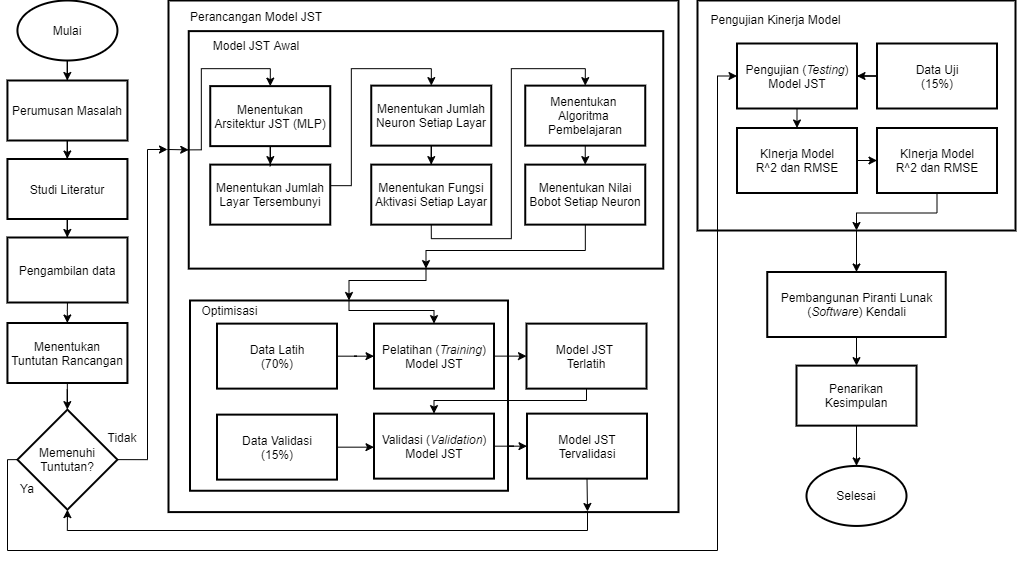
\includegraphics[width=1.5\textwidth]{figures/DiagramPenelitianFull}
%		\caption{Diagram Alir Penelitian Utuh}
%		\label{fig:4:DiagramPenelitianFull}
%	\end{figure}
%\end{landscape}

\subsection{Studi Literatur}
Studi literatur bertujuan untuk mendapatkan pemahaman dalam penyelesaian masalah yang diangkat dalam penelitian ini. Studi literatur juga membantu menegaskan tujuan penelitian sehingga penulis mampu mengetahui perbedaan penelitian ini dengan penelitian terkait yang telah dilakukan sebelumnya. Dari studi literatur yang telah dilakukan maka akan memperjelas tuntutan perancangan dari sistem yang akan dibuat. Informasi yang digunakan bersumber dari berbagai artikel ilmiah, jurnal, skripsi, buku, dan/atau sumber tertulis lainnya yang membahas mengenai sistem kendali lingkungan termal dan/atau jaringan saraf tiruan.

\subsection{Penentuan Tuntutan Rancangan}

Tuntutan pada rancangan ini merujuk pada standar SNI dengan nilai standar suhu udara dijaga pada nilai 25 $\pm$ 1$^{\circ}$C dan nilai kelembapan dinyatakan dalam bentuk \textit{relative humidity} (RH), dijaga pada nilai 60\% $\pm$ 10\%. Sehingga dapat dikatakan bahwa \textit{setpoint} untuk suhu udara bernilai 25$^{\circ}$C dan untuk kelembapan udara (RH) sebesar 60\% dengan kesalahan keadaan tunak tidak melebihi 1$^{\circ}$C (suhu udara) dan 10\% (kelembapan relatif) \cite{SNI-03-06390-2000}. Nilai tersebut akan digunakan sebagai acuan untuk menganalisis perbedaan suhu udara dan kelembaban relatif antara data target dan data prediksi.

\subsection{Pengambilan Data Simulasi IES-VE}
Penelitian ini menggunakan data dari model yang telah dibuat di penelitian sebelumnya berjudul \textbf{Karakterisasi Lingkungan Termal Chamber Iklim Menggunakan Metode Simulasi CFD dengan Perangkat Lunak IES-VE} yang diteliti oleh Ichfan Kurniawan \cite{skripsiIchfan}.  Data tersebut merupakan hasil simulasi pada \textit{software} IES-VE dengan menerapkan beberapa variasi kondisi lingkungan pada model \textit{climate chamber}. Variasi tersebut yaitu kondisi batas lingkungan (radiasi matahari dan suhu bola kering luar / \textit{drybulb temperature}), kondisi AC, dan kondisi \textit{heater}. Variasi kondisi batas lingkungan tersebut diwujudkan dalam pembagian 4 musim dalam 1 tahun, yakni bulan maret, juni, september dan desember. Keluaran dari model IES-VE berupa nilai suhu udara ruang (\textit{air temperature}) \textit{chamber} dan kelembapan relatif (RH) \textit{chamber}. Dari model tersebut didapatkan nilai MAE perhitungan selisih variabel lingkungan termal hasil simulasi dan pengukuran lapangan sebesar 0,8 $\pm$ 0,7$^{\circ}$C untuk suhu udara dan 2,5 $\pm$ 3,8\% untuk kelembaban relatif \cite{skripsiIchfan}. Data yang sudah terkumpul disajikan dalam bentuk tabular yang kemudian diolah dalam program komputer yang dibuat oleh penulis.

\subsection{Identifikasi Sistem menggunakan NARX}
Penelitian ini menggunakan model \textit{plant} yang telah dirancang dari penelitian sebelumnya berjudul \textbf{Pemodelan Lingkungan Termal Sistem \textit{Climate Chamber} dengan Metode Jaringan Saraf Tiruan} yang diteliti oleh Tri Hartanto \cite{skripsiTanto}. Model tersebut merupakan hasil perancangan pada piranti lunak MATLAB dengan menggunakan perangkat NNtools. Model \textit{plant} tersebut memiliki nilai MAE perhitungan antara target dan prediksi sebesar 0,59$^{\circ}$C untuk suhu udara dan 5,44\% untuk kelembapan relatif. Akurasi JST sebesar 96,23\% untuk suhu udara dan 68,90\% untuk kelembapan relatif \cite{skripsiTanto}. Model \textit{plant} tersebut akan diadaptasi oleh penulis dalam melakukan perancangan kendali berbasi jaringan saraf tiruan.

\subsection{Perancangan \textit{Neural Predictive Control}}
Langkah awal untuk melakukan pemodelan kendali yaitu mendefinisikan terlebih dahulu pasangan data input dan data output dari sistem kendali. Untuk mendefinisikan nya perlu menyesuaikan variabel gangguan yang diberikan terhadap sistem dengan variabel keluaran dari AC yang dimana nilai keluaran tersebut dianggap optimal untuk menyesuaikan nilainya terhadap \textit{setpoint}. Nilai output tersebut didapat dari hasil simulasi pada software IES-VE, yang kemudian akan menjadi data latih pada JST yang digunakan pada software MATLAB. Adapun pasangan data kendali dilampirkan pada \textcolor{red}{Lampiran B}.

Pada langkah ini penulis menjabarkan variabel apa saja yang terlibat dalam \textit{plant} terkait sistem kendali yang akan dibuat. Dalam suatu sistem kendali perlu diketahui variabel apa saja yang termasuk dalam kategori \textit{controlled variables}, \textit{manipulated variables}, dan \textit{disturbance variables}. \textit{Controlled variables} adalah variabel akan dikendalikan dalam suatu sistem kendali. \textit{Manipulated variables} adalah variabel yang akan mempengaruhi nilai \textit{controlled variables} melalui \textit{manipulator}/\textit{actuator}. Sementara, \textit{disturbance variables} adalah variabel yang mempengaruhi sistem tetapi perancang tidak memiliki kuasa dalam mengatur nilainya. Hasil dari identifikasi sistem berbentuk diagram blok fungsional. \textit{Manipulated variables} yang akan dikendalikan, yaitu set AC dan set \textit{heater} berada dalam bentuk bilangan bulat. Penulis menggunakan metode yang dijelaskan oleh Shumeet Baluja dalam mengatasi permasalahan estimasi bilangan bulat (tanpa desimal) ini\cite{article26}.

Untuk dapat mengetahui arsitektur JST dengan nilai error sekecil mungkin, dilakukan variasi arsitektur JST. Sama hal nya dngan pemodelan sistem, variasi yang dilakukan juga dengan memvariasikan jumlah layer tersembunyi, jumlah neuron dari masing-masing layer tersembunyi, serta fungsi aktivasi yang digunakan. Algoritma pembelajaran yang digunakan juga sama, yaitu dengan menggunakan Levenberg-Marquadt. Algoritma pembelajaran ini dianggap memiliki kecepatan pembelajaran yang tercepat, serta juga dianggap memiliki konvergensi terbaik untuk mencapai nilai mean square error (MSE) untuk masalah fungsi pendekatan suatu nilai tertentu [12] [13]. Parameter error yang digunakan juga sama, yaitu mean square error (MSE). Adapun proses training pada perancangan kendali juga memiliki proses yang sama dengan perancangan plant. Setelah didapat model yang dianggap baik, maka digunakanlah fungsi genism untuk membangun model di SIMULINK.

\subsection{{Penarikan Kesimpulan}}
Penarikan kesimpulan didapatkan berdasarkan hasil model terbaik yang terpilih dari beberapa percobaan variasi penentuan jumlah \textit{hidden layer} dan/atau jumlah neuron. Kesimpulan menggambarkan bagaimana parameter model yang terpilih sehingga dapat digunakan sebagai sistem kontrol lingkungan termal pada \textit{climate chamber} DTNTF FT UGM.

\section{Rencana Analisis Hasil Penelitian}
Data yang diperoleh dari hasil perancangan jaringan saraf tiruan berupa data nilai RMSE dari proses pelatihan, proses validasi, dan proses pengujian. Data nilai RMSE pengujian mewakili tingkat keakuratan model yang divariasikan. Semakin kecil nilai RMSE, semakin tinggi akurasi yang dihasilkan oleh model. Selain itu, tingkat konsistensi model juga perlu diuji dengan menggunakan nilai standar deviasi dari nilai \textit{error} pengujian. Model yang memiliki tingkat konsistensi yang tinggi merupakan model dengan standar deviasi \textit{error} paling rendah.

Model terpilih merupakan model yang memiliki tingkat akurasi dan konsistensi yang tinggi. Tingkat akurasi model dapat diwakili dengan nilai rerata RMSE pengujian. Sedangkan tingkat konsistensi diwakili dengan nilai standar deviasi RMSE pengujian terkecil. Semakin kecil nilai rata-rata dan standar deviasi RMSE pengujian, maka model yang dipilih semakin akurat dan konsisten.

Setelah penulis memilih model yang akurat dan konsisten, model tersebut diuji kinerjanya dengan cara membandingkan nilai prediksi dari model terhadap nilai target yang sebenarnya. Kemudian, pengujian model berlanjut dengan mengurangi keluaran jaringan yang akan diprediksi untuk melihat pengaruh jumlah keluaran jaringan terhadap \textit{error} yang dihasilkan.
\chapter{HASIL DAN PEMBAHASAN}
\label{hasil-dan-pembahasan}
Bangunan yang dijadikan objek pengendalian adalah \textit{Climate Chamber} DTNTF FT UGM. Dalam bab ini, akan dibahas mengenai hasil sistem kendali sesuai dengan langkah-langkah yang dijelaskan pada Bab IV dengan memvariasikan berbagai macam masukan, kemudian mengetahui keluarannya. Variasi masukan dan keluaran akan dimodelkan dengan model jaringan saraf tiruan untuk mendapatkan parameter-parameter model yang dapat mengendalikan sistem bangunan.

\section{Hasil Pengambilan Data Simulasi IES-VE}
Hasil-hasil yang disajikan bukan data mentah, melainkan data yang telah diolah dengan proses sebagaimana tercantum dalam pasal ``Rencana analisis hasil'' Bab IV tentang ``Pelaksanaan Penelitian''.
\subsection{Kondisi \textit{Climate Chamber}}
\subsection{Hasil Rancangan Skenario}
\subsection{Hasil Simulasi IES-VE}

\section{Pembangunan Arsitektur JST}
Data dibagi menjadi 3 bagian, yakni 70\% data pelatihan, 15\% data validasi, dan 15\% data pengujian. Model JST menggunakan arsitektur \textit{multilayer perceptron} dengan jumlah neuron sebanyak $x_1$ di lapisan tersembunyi 1, $x_2$ di lapisan tersembunyi 2, dan $x_3$ di lapisan tersembunyi 3.

\section{Analisis Kinerja Arsitektur JST yang terpilih}

Persamaan ditulis rata tengah dan nomor persamaan ditulis rata kanan. Nomor persamaan
diurutkan dengan format (nomor\_bab.nomor\_persamaan). Contoh dapat dilihat pada Persamaan \eqref{eq:1}.

\begin{equation}
    \dfrac{Dv}{Dt} = \dfrac{\partial v}{\partial t} + \nabla \cdot \mathbf{uu}
\label{eq:1}
\end{equation}


\chapter{KESIMPULAN DAN SARAN}
\label{kesimpulan-dan-saran}

\section{Kesimpulan}
Rancangan kontroler berbasis jaringan saraf tiruan memiliki nilai \textit{steady-state error} sebesar 0,18$^\circ$C untuk suhu ruang. Kontroler berbasis jaringan saraf tiruan yang dihasilkan dibangun dengan pembagian data 80\% data latih, 10\% data validasi, dan 10\% data uji. Model Kontroler JST menggunakan fungsi aktivasi \textit{hyperbolic tangent} dengan algoritma pembelajaran Levenberg-Marquardt. Model Kontroler JST terdiri dari 1 lapisan tersembunyi dengan 35 neuron. Akan tetapi, kontroler tidak mampu mengendalikan suhu ruang \textit{climate chamber} di atas nilai \textit{set point} 26$^\circ$C dikarenakan data lingkungan termal dari Model IES-VE kurang mewakili kondisi sistem pada suhu yang tinggi.

\section{Saran}

%Berikut merupakan saran-saran untuk pengembangan kontroler ini agar menjadi lebih baik pada penelitian-penelitian selanjutnya:
\begin{enumerate}
	\item Disarankan untuk melakukan validasi model di nilai suhu yang tinggi terlebih dahulu apabila menggunaan model IES-VE yang serupa.
	\item Memperkaya data pelatihan model JST menggunakan data pengukuran langsung pada \textit{climate chamber} dalam merancang kontroler JST.
	\item Menambahkan semacam \textit{manipulator}/aktuator pada \textit{climate chamber} untuk memanipulasi kelembapan relatif ruang secara langsung seperti penelitian yang dilakukan oleh Moon \cite{paper22JJkim}. Contoh: \textit{humidifier} dan \textit{dehumidifier}.
	\item Menambahkan variabel kontrol lainnya ke dalam rancangan kontroler, seperti kecepatan angin, suhu radian, RH lingkungan, dsb.
\end{enumerate}


\begin{singlespace}
\bibliographystyle{skripsi}
\bibliography{pustaka}
\end{singlespace}

% beri comment pada bagian ini jika tidak ada lampiran.
%%%%%%%
\appendix
\addappheadtotoc
\appendixpage
\chapter{Data Penelitian}

\section{Data Simulasi IES-VE}
Data penelitian ini dapat diakses di \textit{http://bit.ly/DataSkripsiS1Ridhan}

\begin{table}[!h]
	\caption{Data Simulasi IES-VE}
	\label{tbl:A:DataSkripsiRidhan}
	\centering
	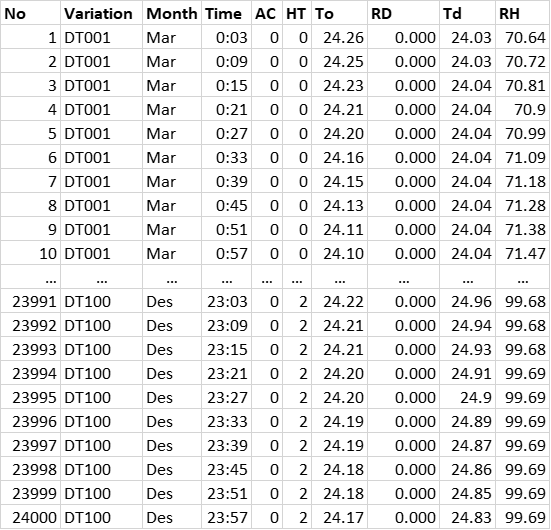
\includegraphics[width=0.75\textwidth]{figures/DataSkripsiRidhan}
\end{table}
\vspace{3em}
\break
\break

\section{Bobot-bobot Model JST Kontroler}
\begin{table}[!h]
	\caption{Bobot-bobot Model JST Kontroler}
	\label{tbl:A:BobotKontroler}
	\centering
	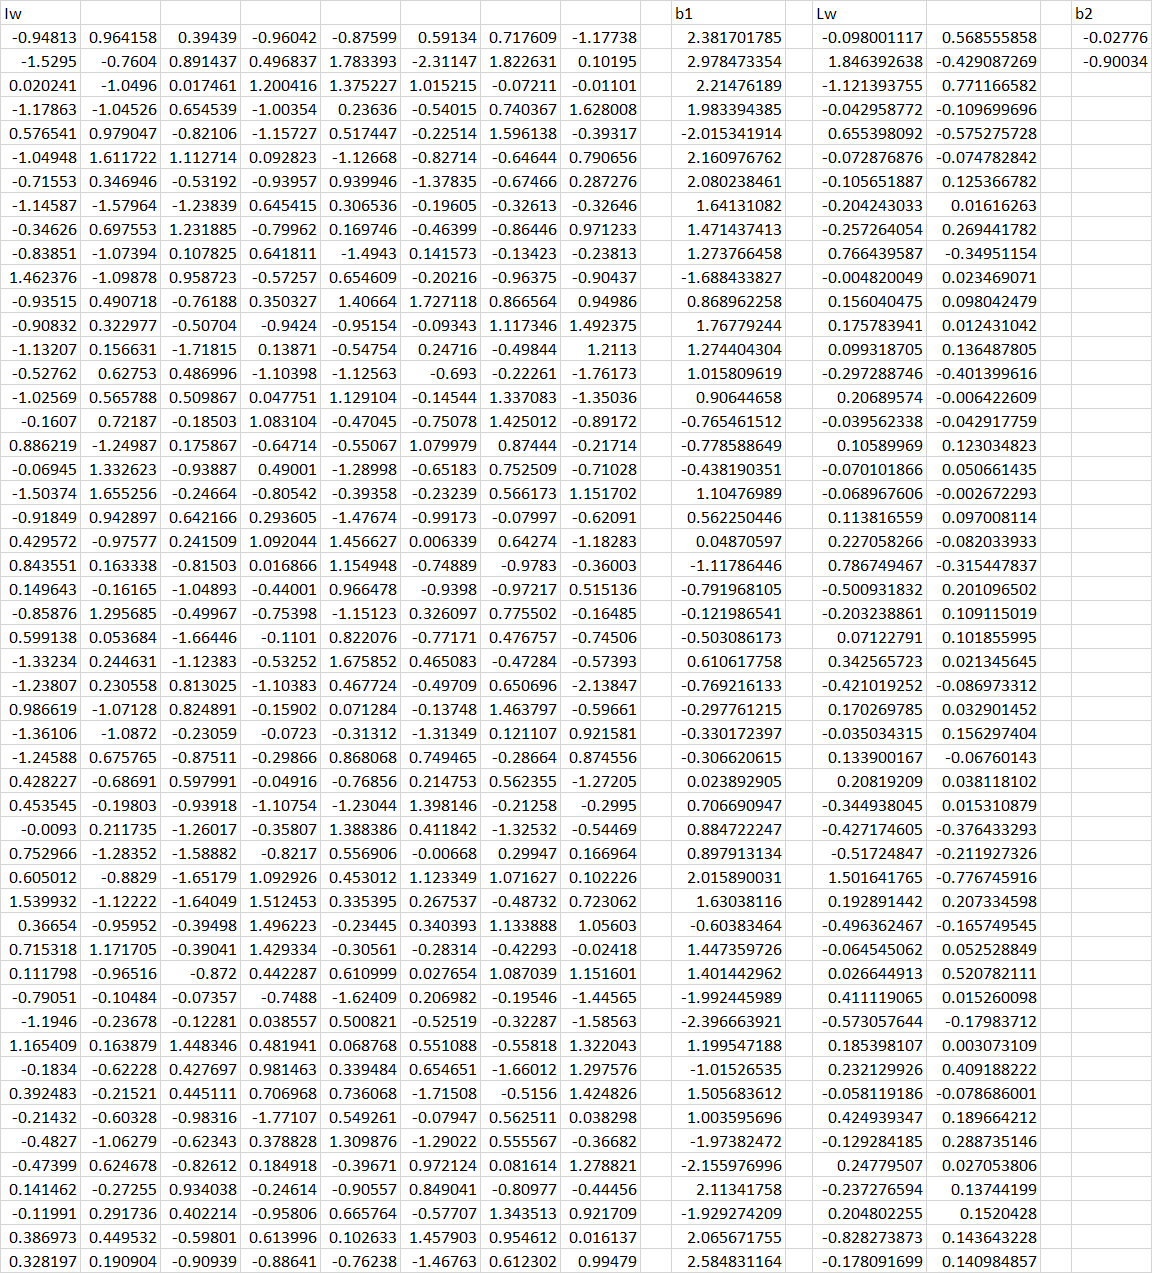
\includegraphics[width=1\textwidth]{figures/BobotKontroler}
\end{table}
\vspace{1em}
\break

\section{Hasil Simulasi Sistem Kontrol}
\begin{table}[!h]
	\caption{Hasil Simulasi Sistem Kontrol}
	\label{tbl:A:HasilSimulasiKontrol1}
	\centering
	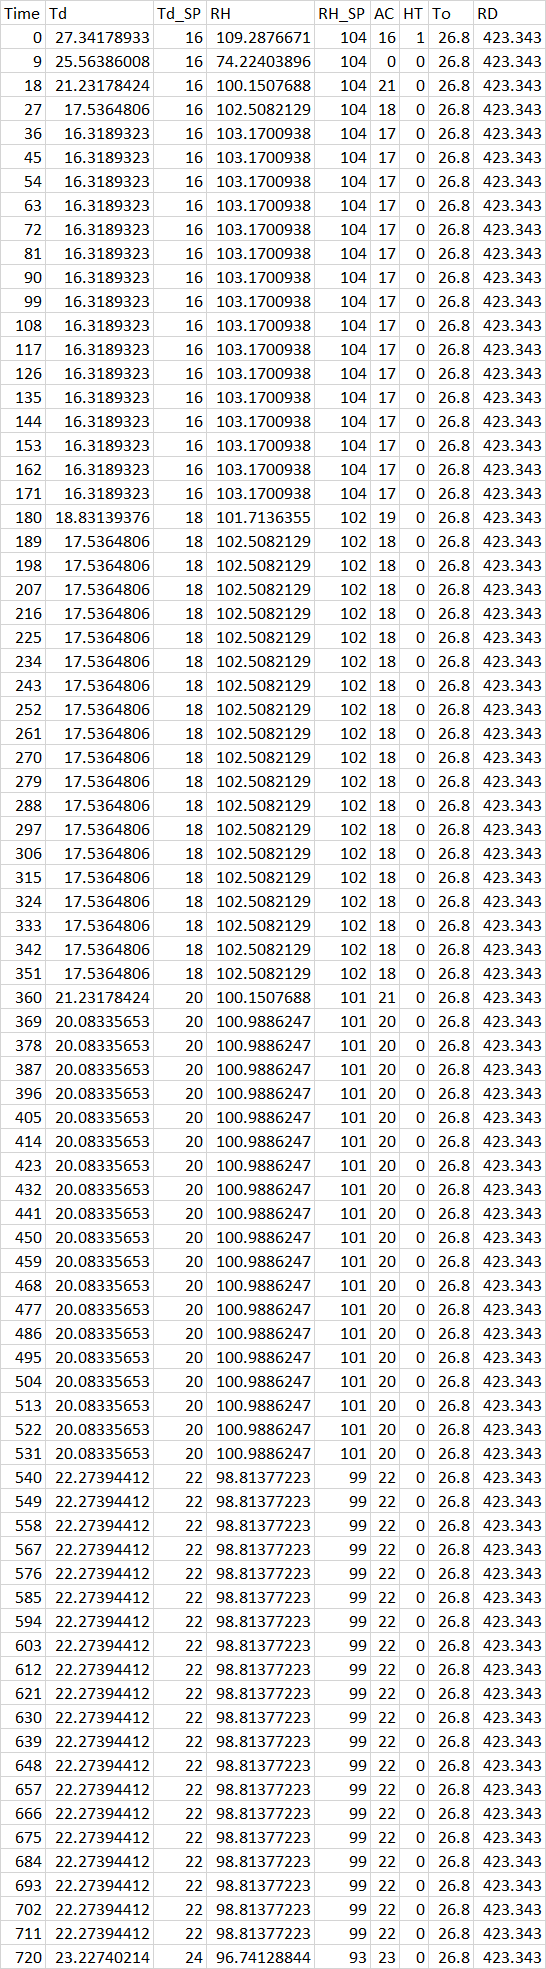
\includegraphics[width=0.34\textwidth]{figures/HasilSimulasiSimulink1}
\end{table}
\break

\section{Hasil Simulasi Sistem Kontrol (lanjutan 2)}
\begin{table}[!h]
	\caption{Hasil Simulasi Sistem Kontrol}
	\label{tbl:A:HasilSimulasiKontrol2}
	\centering
	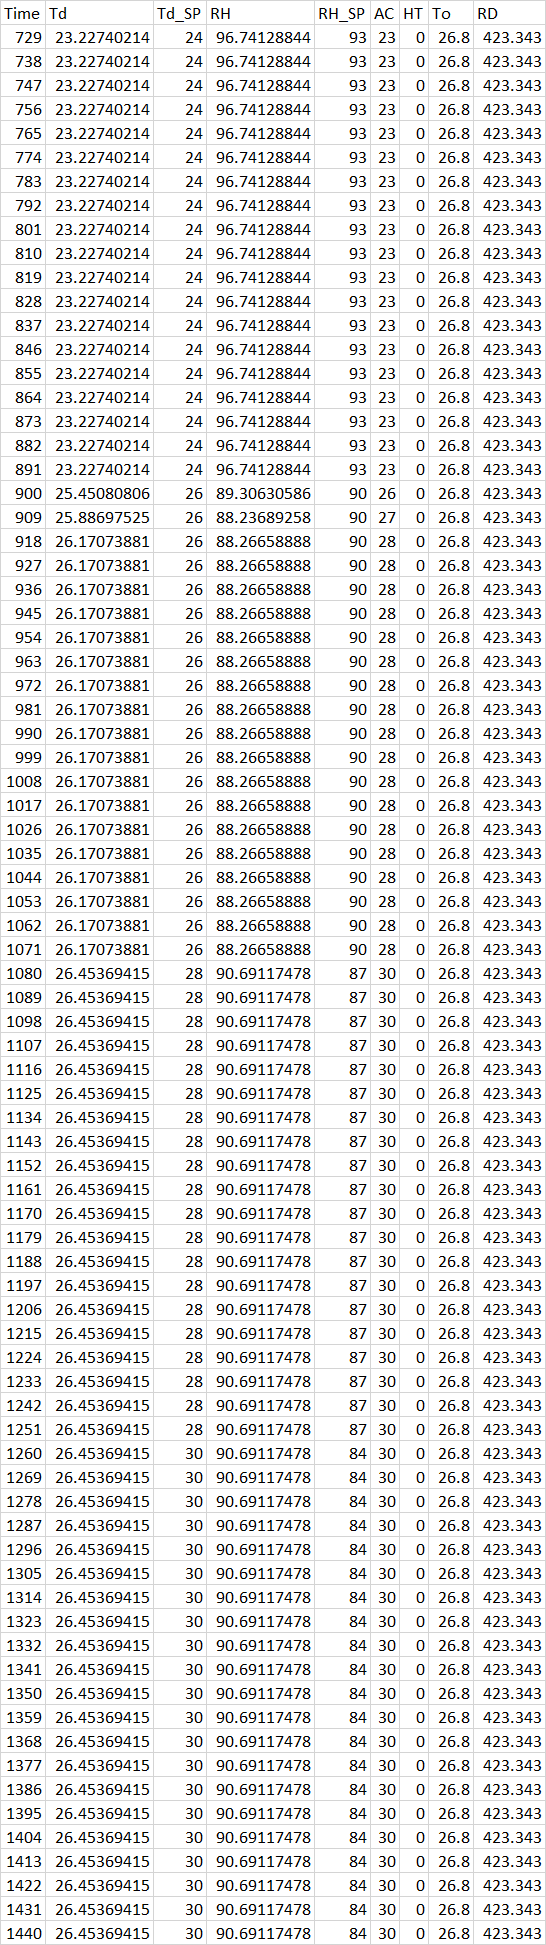
\includegraphics[width=0.35\textwidth]{figures/HasilSimulasiSimulink2}
\end{table}
\break

\section{Hasil Simulasi Sistem Kontrol (lanjutan 3)}
\begin{table}[!h]
	\caption{Hasil Simulasi Sistem Kontrol}
	\label{tbl:A:HasilSimulasiKontrol3}
	\centering
	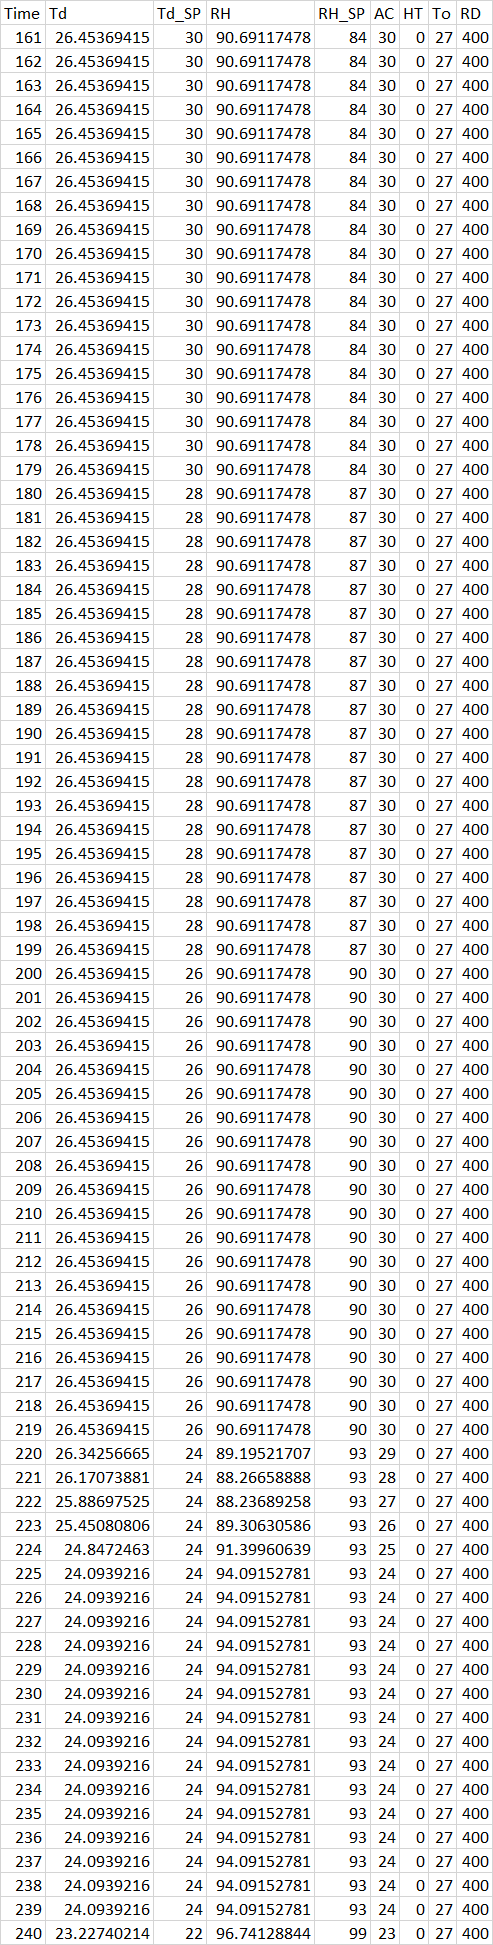
\includegraphics[width=0.35\textwidth]{figures/HasilSimulasiSimulink3}
\end{table}
\break

\section{Hasil Simulasi Sistem Kontrol (lanjutan 4)}
\begin{table}[!h]
	\caption{Hasil Simulasi Sistem Kontrol}
	\label{tbl:A:HasilSimulasiKontrol4}
	\centering
	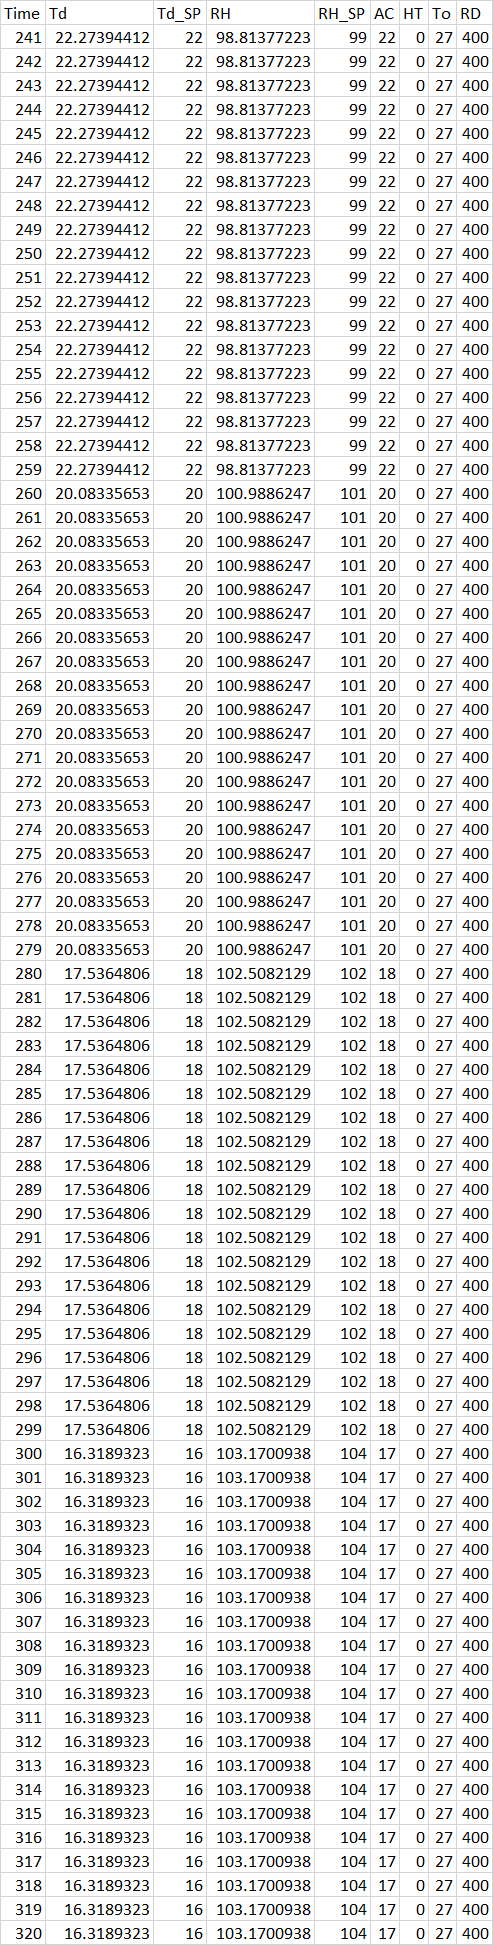
\includegraphics[width=0.35\textwidth]{figures/HasilSimulasiSimulink4}
\end{table}
\chapter{Listing Program}
\singlespacing

\lstset{language=Matlab,%
	%basicstyle=\color{red},
	breaklines=true,%
	morekeywords={matlab2tikz},
	keywordstyle=\color{blue},%
	morekeywords=[2]{1}, keywordstyle=[2]{\color{black}},
	identifierstyle=\color{black},%
	stringstyle=\color[rgb]{0.5,0,0.5},
	commentstyle=\color[rgb]{0.13,0.54,0.13},%
	showstringspaces=false,%without this there will be a symbol in the places where there is a space
	numbers=left,%
	numberstyle={\tiny \color{black}},% size of the numbers
	numbersep=9pt, % this defines how far the numbers are from the text
	emph=[1]{for,end,break},emphstyle=[1]\color{red}, %some words to emphasise
	%emph=[2]{word1,word2}, emphstyle=[2]{style},    
}

\section{Kode Sumber Program Model JST Kontroler}
\begin{lstlisting}
% Import Data
data = xlsread('DataSkripsiS1Ridhan.xlsx');
Control_Input = data(:,5:6)';
Plant_Output  = data(:,9:10)';

% Set up Data
Yp = Plant_Output;  % Plant Output
u  = Control_Input; % Manipulated Variable
[~,datasize] = size(Yp);
clear data Control_Input Load_var Plant_Output;

% Feature Scaling
parY = [30.31, 100; 16, 55.84];
[Yp, ~] = MinMaxScaler(Yp',parY);
Yp = Yp';
clear parY;

% ANN Input Output
normal = 2:datasize;
delay = 1:datasize-1;
X  = [Yp(:,delay);Yp(:,normal);u(:,delay)]; % Feature
T  = u(:,normal); % Target
clear Yp u normal delay;

% Create a Fitting Network
hiddenLayerSize = 35;
netC = feedforwardnet(hiddenLayerSize);

% Choose a Training Function
netC.trainFcn = 'trainlm'; % Levenberg-Marquardt backpropagation.

% Choose Input and Output Pre/Post-Processing Functions
% For a list of all processing functions type: help nnprocess
netC.input.processFcns = {'removeconstantrows','mapminmax'};
netC.output.processFcns = {'removeconstantrows','mapminmax'};

% Setup Division of Data for Training, Validation, Testing
% For a list of all data division functions type: help nndivision
netC.divideFcn = 'dividerand';  % Divide data randomly
netC.divideMode = 'sample';  % Divide up every sample
netC.divideParam.trainRatio = 80/100;
netC.divideParam.valRatio = 10/100;
netC.divideParam.testRatio = 10/100;

% Choose activation functions
netC.layers{1}.transferFcn = 'tansig';
netC.layers{2}.transferFcn = 'purelin';

% Choose a Performance Function
% For a list of all performance functions type: help nnperformance
netC.performFcn = 'mse';  % Mean Squared Error

% Choose Plot Functions
% For a list of all plot functions type: help nnplot
netC.plotFcns = {'plotperform','plottrainstate','ploterrhist', ...
'plotregression', 'plotfit'};

% Train the Network
[netC,tr] = train(netC,X,T);

% Test the Network
u = netC(X);

% Network Performance
e = gsubtract(T,u);
MAE = mean(abs(e),2);
MAE_All = mean(MAE);
MSE = mean(e.^2,2);
MSE_All = perform(netC,T,u);
MSE_Relatif = mean(e/T,2);
MSE_Std = std(e,0,2);

% Correlation Coefficient
[~,~,R_AC] = postreg(T(1,:),u(1,:));
[~,~,R_HT] = postreg(T(2,:),u(2,:));
[~,~,R_All] = postreg(T,u);
R = [R_AC,R_HT];
clear R_AC R_HT;

% Recalculate Training, Validation and Test Performance
trainTargets = T .* tr.trainMask{1};
valTargets = T .* tr.valMask{1};
testTargets = T .* tr.testMask{1};
All_MSETrain = perform(netC,trainTargets,u);
All_MSEVal = perform(netC,valTargets,u);
All_MSETest = perform(netC,testTargets,u);
\end{lstlisting}
\vspace{1em}

\section{Fungsi Min Max Scaler}
\begin{lstlisting}
function [newx, par] = MinMaxScaler(x,parx)
  if (parx == 0)
    newx = ( x - min(x) ) ./ ( max(x) - min(x) );
    par  = [[max(x)]; [min(x)]];
  else
    maxx  = parx(1,:);
    minx  = parx(2,:);
    newx  = ( x - minx ) ./ ( maxx - minx );
    par   = parx;
  end
end
\end{lstlisting}
\break

\section{Fungsi Kuantisasi AC}
\begin{lstlisting}
function y = QuantizationAC(u)
  AC  = round(u);
  if (AC < 12)
    y = 0;
  elseif (AC <= 16)
    y = 16;
  elseif (AC >= 30)
    y = 30;
  else
    y = AC;
end
\end{lstlisting}
\vspace{1em}

\section{Fungsi Kuantisasi Heater}
\begin{lstlisting}
function y = QuantizationHT(u)
  HT = round(u);
  if (HT < 1)
    y = 0;
  elseif (HT > 2)
    y = 2;
  else
    y = HT;
end
\end{lstlisting}
\vspace{1em}

\section{Fungsi Penskalaan Suhu Ruang}
\begin{lstlisting}
function y = ScalerTd(u)
  maxTd  = 30.31;
  minTd  = 16;
y = ( u - minTd ) ./ ( maxTd - minTd );
\end{lstlisting}
\vspace{1em}

\section{Fungsi Penskalaan Kelembapan Relatif}
\begin{lstlisting}
function y = ScalerRH(u)
  maxRH  = 100;
  minRH  = 55.84;
y = ( u - minRH ) ./ ( maxRH - minRH );
\end{lstlisting}
\chapter{About \LaTeX}

\section{Package yang Diperlukan}
Pastikan packages berikut ini telah terinstall pada sistem \LaTeX Anda.

\begin{enumerate}
    \item indentfirst

\item setspace
\item times
\item graphicx
\item latexsym
\item supertabular
\item multirow
\item rotating
\item appendix
\item ifthen
\item nomencl
\item tocloft
\item enumitem
\item caption
\item color
\item listings
\item subfigure
\item url
\item science.sty (scientificpaper)
\item abstract
\end{enumerate}

Sebagian besar dari package tersebut telah terinstall secara default. Apabila ternyata belum terinstall, bisa diunduh dari CTAN.

\section{File yang diubah isinya oleh penulis}
File-file berikut ini diubah oleh penulis sesuai dengan tugas akhir yang dikerjakan
\begin{enumerate}
    \item \texttt{data\_skripsi.tex} \\ berisi data mengenai skripsi, misal judul, nama penguji, nama pembimbing, tanggal ujian, dan sebagainya.
    \item \texttt{persembahan.tex} \\ berisi kepada siapa skripsi ini dipersembahkan (\textit{dedicated}). Halaman persembahan boleh tidak ada. Jika demikian, beri comment pada file \texttt{muka\_skripsi.tex}.
    \item \texttt{motto.tex} \\ berisi moto penulis. Halaman moto boleh tidak ada.  Jika demikian, beri comment pada file \texttt{muka\_skripsi.tex}.
    \item \texttt{prakata.tex} \\ berisi kata pengantar.
    \item \texttt{lambang.tex} \\ berisi input untuk menyusun daftar lambang.
    \item \texttt{abstrakind.tex} \\ berisi abstrak dalam bahasa Indonesia.
    \item \texttt{abstrakeng.tex} \\ berisi abstrak dalam bahasa Inggris.
    \item \texttt{Bab1.tex, Bab2.tex, ..., Bab6.tex} \\ isi dari masing-masing bab.
    \item \texttt{app1.tex, app2.tex, ...} \\ isi dari lampiran. Beri comment pada file \texttt{skripsi.tex} jika tidak terdapat lampiran.
    \item \texttt{pustaka.bib} \\ isi dengan pustaka atau acuan yang digunakan.
\end{enumerate}


\section{Menghasilkan file PDF}
Template ini dibuat secara langsung menggunakan \texttt{PDFLatex}. Jika Anda menggunakan jalur ``biasa'', maka alur yang digunakan adalah:
\begin{equation*}
    latex \longrightarrow dvips \longrightarrow pstopdf
\end{equation*}

Untuk menghasilkan Daftar Lambang, gunakan perintah berikut:
\begin{equation*}
    makeindex \quad skripsi.nlo\quad -s\quad nomencl.ist\quad -o\quad skripsi.nls
\end{equation*}

Jangan lupa untuk me-run latex sekali lagi. Jadi urutan perintahnya adalah
\begin{enumerate}
    \item latex
    \item latex
    \item makeindex 
    \item latex
\end{enumerate}

Jika Anda tidak mengubah Daftar Lambang (dengan mengubah file ``lambang.tex''), maka perintah \texttt{makeindex} tidak perlu dilakukan.




%%%%%%
\end{document}

